% This is part of Le Frido
% Copyright (c) 2006-2025
%   Laurent Claessens, Carlotta Donadello
% See the file fdl-1.3.txt for copying conditions.


%+++++++++++++++++++++++++++++++++++++++++++++++++++++++
\section{Applications analytique entre espaces de Banach}
%+++++++++++++++++++++++++++++++++++++++++++++++++++++++

%-------------------------------------------------------
\subsection{Série de puissance}
%----------------------------------------------------


\begin{definition}[\cite{BIBooTIAZooFwCEtZ}]	\label{DEFooIXGBooPgJTzB}
	Soient des espaces de Banach\footnote{Définition \ref{DefVKuyYpQ}.} \( E\) et \( F\).
	Une \defe{série de puissance}{série de puissance} sur \( E\) à valeurs dans \( F\) est une application de la forme
	\begin{equation}
		x\mapsto \sum_{n=0}^{\infty}\alpha_n(x)
	\end{equation}
	où les \( \alpha_n\) sont des applications
	\begin{enumerate}
		\item
		      \( n\)-multilinéaire, c'est-à-dire \( \alpha_n\in \aL_n(E,F)\) (définition \ref{DefFRHooKnPCT}),
		\item
		      symétrique,
		\item
		      continue.
	\end{enumerate}
	En termes de notations, nous posons
	\begin{equation}
		\alpha_n(x)=\alpha(x,\ldots,x)=\alpha_nx^n.
	\end{equation}
	Notons toutefois que la dernières notation est particulièrement vicieuse parce que, si \( E\) est un espace de Banach, il n'y a pas de sens à multiplier des éléments de \( E\) entre eux.

	Notons aussi que \( \alpha_0\) est une application \( 0\)-multilinéaire, c'est-à-dire juste un élément de \( F\).
\end{definition}

\begin{definition}[\cite{BIBooTIAZooFwCEtZ}]	\label{DEFooZUYHooDwwRfp}
	Une série de puissance qui est une somme finie est un \defe{polynôme}{polynôme sur un espace de Banach}.
\end{definition}


\begin{normaltext}
	Nous avons deux définitions de polynômes. Une sur les espaces de Banach qui ne s'applique pas aux anneaux, et une sur les anneaux (\ref{DEFooFYZRooMikwEL}) qui ne s'applique pas aux espaces de Banach.

	Entre les deux, je vous propose d'espérer que les deux définitions coïncident sur les espaces de Banach qui sont en même temps des anneaux. Typiquement \( \eR\).
	%TODOooZPEMooOwmONe. Le faire. C'est dans la liste.
\end{normaltext}

\begin{definition}[\cite{MonCerveau}]	\label{DEFooCAWCooWHLpwl}
	Soit une série de puissance \( \sum_{n=0}^{\infty}\alpha_k(x)\). Le \defe{rayon de convergence}{rayon de convergence} de \( (\alpha_k)_{k\in \eN}\) est le nombre
	\begin{equation}
		R=\sup\{ r\in \eR^+\tq \text{la suite \( (\alpha_kr^k)_{n\in \eN}\) est bornée dans \( \aL_k(E,F)\)} \}.
	\end{equation}
\end{definition}


%-------------------------------------------------------
\subsection{Applications analytiques}
%----------------------------------------------------

\begin{definition}[\cite{BIBooTIAZooFwCEtZ}]	\label{DEFooAIHMooKbWsBt}
	Soient deux espaces de Banach \( E\) et \( F\). Une application \(f \colon E\to F  \) définie sur un voisinage de \( x_0\in E\) est \defe{analytique}{analytique entre espaces de Banach} en \( x_0\) si il existe un voisinage \( U\) de \( x_0\) sur lequel nous avons
	\begin{equation}		\label{EQooWATIooCCmlbT}
		f(x)=\sum_{k=0}^{\infty}\alpha_k(x-x_0)^k
	\end{equation}
	avec les conditions
	\begin{enumerate}
		\item
		      Pour chaque \( k\in \eN\), l'application \( \alpha_k\) est une forme \( k\)-multilinéaire, continue et symétrique
		\item
		      La notation \( \alpha_kx^k=\alpha_k(x,\ldots,x)\).
		\item
		      Pour chaque \( x\in U\), nous avons
		      \begin{equation}	\label{EQooQYBGooKyoNHA}
			      \sum_{k=0}^{\infty}\| \alpha_k \|\| x-x_0 \|^k<\infty
		      \end{equation}
		      où \( \| \alpha_k \|\) est la norme de \( \alpha_k\) en tant qu'application \( k\)-multilinéaire, définition \ref{DEFooTAUWooNDJJEO}.
	\end{enumerate}
\end{definition}

\begin{normaltext}
	Notez que la condition \eqref{EQooQYBGooKyoNHA} n'est pas la convergence absolue de \( \sum_n\alpha_n(x)\) qui aurait été la condition \( \sum_n\| \alpha_n(x) \|_F<\infty\) ni la convergence normale qui aurait été \( \sum_n\| \alpha_n \|<\infty\).
\end{normaltext}

\begin{proposition}[Critère d'Abel\cite{MonCerveau}]	\label{PROPooHCYXooHlUEuV}
	Soit une série entière \( \sum_{n=0}^{\infty}\alpha_k(x)\) de rayon de convergence \( R\).

	\begin{enumerate}
		\item		\label{ITEMooVAOTooELMOlK}
		      Si \( \| x \|<R\) alors
		      \begin{equation}
			      \sum_{n=0}^{\infty}\| \alpha_n \|\| x \|^n<\infty.
		      \end{equation}
		      Autrement dit : une série entière est analytique à l'intérieur de son disque de convergence.
		\item	\label{ITEMooEEVMooVeiHyY}
		      Si \( \| x \|>R\) alors
		      \begin{equation}
			      \sum_{n=0}^{\infty}\| \alpha_n \|\| x \|^n=\infty.
		      \end{equation}
		      Autrement dit : une série entière n'est pas analytique à l'extérieur de son disque de convergence.
	\end{enumerate}
\end{proposition}

\begin{proof}
	Nous considérons un \( r\in \eR\) satisfaisant \( \| x \|<r<R\), et nous considérons un majorant \( M\) pour \( \| \alpha_n \|r^n\). Nous avons alors
	\begin{equation}
		\| \alpha_n \|\| x \|^n=\| \alpha_n \|r^n\left( \frac{ \| x \| }{ r } \right)^n\leq M\left( \frac{ \| x \| }{ r } \right)^r.
	\end{equation}
	Donc la suite \( \| \alpha_n \|\| x \|\) est majorée par la suite \( M(\| x \|/r)^r\) dont la série est convergente en tant que série géométrique (proposition \ref{PROPooWOWQooWbzukS}\ref{ITEMooVZHKooNGpDkx}).

	Si \( \| x \|>R\) alors la suite \( \| \alpha_k \|\| x \|^r\) n'est pas bornée. En tant que série de termes positifs non bornés nous avons \( \sum_{n=0}^{\infty}\| \alpha_n \|\| x \|^n=\infty\).
\end{proof}

\begin{lemma}[\cite{MonCerveau}]	\label{LEMooZDPSooXxPkYs}
	Soit une application \(f \colon E\to F  \) analytique sur \( \overline{B(x_0,R)}\) s'écrivant sous la forme
	\begin{equation}
		f(x)=\sum_{k=0}^{\infty}a_k(x-x_0)
	\end{equation}
	avec \( a_k(x)=\sum_{\alpha\in\Lambda_k}a_{\alpha}x^{\alpha}\).

	Il existe \( C>0\) tel que pour tout \( \epsilon>0\) il existe \( N\in \eN\) tel que pour tout \( k\geq N\) nous ayons
	\begin{equation}
		| a_{\alpha} |<\frac{ \epsilon }{ C }R^{-k}.
	\end{equation}
\end{lemma}

\begin{proof}
	Soit \( \epsilon>0\). Nous considérons \( x\in B(x_0,R)\), en choisissant de telle sorte à avoir \( \| x-x_0 \|=R\). Nous avons donc, par définition d'une application analytique :
	\begin{equation}
		\sum_{k=0}^{\infty}\| a_k \|\| x-x_0 \|^k=\sum_{k=0}^{\infty}\| a_k \|R^k<\infty.
	\end{equation}
	Par la proposition \ref{PROPooYDFUooTGnYQg}, il existe alors \( N\) tel que si \( k\geq N\) alors \( \| a_k \|R^k<\epsilon\). Vu que \( \max_{\alpha\in\Lambda_k}| a_{\alpha} |\) est une norme (lemme \ref{LEMooORANooRLJYWw}) et que toutes les normes sont équivalentes, il existe \( C'>0\) tel que  \( C| a_{\alpha} |R^k<\epsilon\) et donc en posant \( C=1/C'\) nous avons bien
	\begin{equation}
		| a_{\alpha} |<C\epsilon R^{-k}.
	\end{equation}
\end{proof}


\begin{proposition}[\cite{MonCerveau}]	\label{PROPooMGWOooTeCDRk}
	Toute application linéaire est analytique.
\end{proposition}

\begin{proof}
	Si \(f \colon E\to F  \) est linéaire, alors \( f(x)=\sum_{n=0}^{\infty}\alpha_n(x)\) avec \( \alpha_k(x)=0\) pour \( k\neq 1\) et \( \alpha_1(x)=f(x)\).
\end{proof}

\begin{theorem}[\cite{BIBooTIAZooFwCEtZ}]	\label{THOooNBNFooMsAorH}
	Soient des espaces de Banach \( E\) et \( F\) sur \( \eC\). Soient des applications \( \alpha_n\in\aL(E,F)\). Nous supposons que \( \{ \alpha_n(x) \}\) est borné. Nous posons \( z=tx\) avec \( | t |<1\). Alors
	\begin{equation}
		\sum_{n=0}^{\infty}\alpha_n(z)
	\end{equation}
	converge absolument.
\end{theorem}

\begin{proof}
	Par hypothèse, il existe \( K\in\eR\) tel que \( \| \alpha_n(x) \|<K\) pour tout \( n\). Alors nous avons
	\begin{equation}
		\| \alpha_n(z) \|=\| \alpha_n(tz,\ldots,tz) \|=\| t^n\alpha_n(z,\ldots,z) \|\leq | t |^nK.
	\end{equation}
	Vu que \( | t |<1\), la série \( \sum_{n=0}^{\infty}K| t |^n\) converge (proposition \ref{PROPooWOWQooWbzukS}\ref{ITEMooAFAMooGuXqBm}). Donc la série \( \sum_k\| \alpha_n(z) \|\) converge par le critère de comparaison\footnote{Lemme \ref{LemgHWyfG}\ref{ITEMooBBWTooYDHnuH}.}
\end{proof}

\begin{normaltext}		\label{NORMooQDCKooXHtrHQ}
	Dans la suite, nous devons faire appel à quelques astuces de notations. Si \( \alpha\in\aL_n\), nous notons \( \alpha(x)\) pour \( \alpha(x,\ldots,x)\).

	Si \( \alpha\in \aL_{k+n}(E,F)\) est symétrique, alors nous notons \( \alpha x^n\) l'élément de \(\aL_k(E,F) \) donné par
	\begin{equation}
		(y_1,\ldots,y_k)\mapsto \alpha(x,\ldots,x,y_1,\ldots,y_n).
	\end{equation}
	Notons au passage que l'ordre n'est pas important parce que \( \alpha\) est symétrique.
\end{normaltext}


\begin{theorem}[\cite{BIBooTIAZooFwCEtZ,BIBChatGPT}]	\label{THOooHSXLooMCzTTD}
	Soient des espaces de Banach \( E\) et \( F\). Nous supposons que la série de puissance
	\begin{equation}
		\begin{aligned}
			f\colon E & \to F                                   \\
			x         & \mapsto \sum_{n=0}^{\infty}a_n(x-x_0)^n
		\end{aligned}
	\end{equation}
	ait un rayon de convergence \( r_0>0\).

	Nous posons\footnote{Voir la notation expliquée en \ref{NORMooQDCKooXHtrHQ}.}
	\begin{equation}		\label{EQooXVAIooOXGaQz}
		b_k=\sum_{n=0}^{\infty}\binom{n+k}{n}a_{n+k}(x_1-x_0)^n\in\aL_k(E,F),
	\end{equation}
	Alors :
	\begin{enumerate}
		\item		\label{ITEMooWBTAooGrKzpo}
		      \( f\) est analytique\footnote{Définition \ref{DEFooAIHMooKbWsBt}.} en tout point de \( B(x_0,r)\),
		\item		\label{ITEMooOPLBooTZZOOx}
		      Pour tout \( x\in B(x_1,r_1)\) nous avons
		      \begin{equation}
			      f(x)=\sum_{k=0}^{\infty}b_k(x-x_1)^k.
		      \end{equation}
		\item		\label{ITEMooNTPIooXpKePf}
		      La série
		      \begin{equation}
			      \sum_{k=0}^{\infty}b_k(x-x_1)^k
		      \end{equation}
		      a un rayon de convergence \( r_1\geq r_0-\| x_1-x_0 \|\).
	\end{enumerate}
\end{theorem}

\begin{proof}
	En plusieurs parties.
	\begin{subproof}
		\spitem[Pour \ref{ITEMooWBTAooGrKzpo}]
		%-----------------------------------------------------------
		C'est le critère d'Abel \ref{PROPooHCYXooHlUEuV}\ref{ITEMooVAOTooELMOlK}.
		\spitem[Pour \ref{ITEMooOPLBooTZZOOx}]
		%-----------------------------------------------------------
		Soit \( x_1\in B(x_0,r)\). Notons \( h=x_1-x_0\), de telle sorte que \( x-x_0=(x-x_1)+h\). En appliquant la multilinéarité de \( \alpha_n\), nous voyons que le binôme de Newton \ref{PropBinomFExOiL} fonctionne aussi bien :
		\begin{equation}
			\alpha_n\big( (x-x_1)+h \big)=\sum_{k=0}^n\binom{ n }{ k }\alpha_n\big( h^{n-k},(x-x_1)^k \big).
		\end{equation}
		Nous pouvons permuter les deux sommes avec le lemme \ref{LEMooKMCIooItDMRo} :
		\begin{subequations}
			\begin{align}
				f(x) & =\sum_{n=0}^{\infty}\alpha_n\big( (x-x_1)+h \big)                                                 \\
				     & =\sum_{n=0}^{\infty}\sum_{k=0}^n\binom{ n }{ k }\alpha_n\big( h^{n-k},(x-x_1)^k \big)             \\
				     & =\sum_{k=0}^{\infty}\sum_{n=k}^{\infty}\binom{ n }{ k }\alpha_n\big( h^{n-k},(x-x_1)^k \big)      \\
				     & =\sum_{k=0}^{\infty}\left( \sum_{n=k}^{\infty}\binom{ n }{ k }\alpha_n(h^{n-k}) \right)(x-x_1)^k.
			\end{align}
		\end{subequations}
		Donc en posant \( \beta_k=\sum_{n=k}^{\infty}\binom{ n }{ k }\alpha_n(h^{n-k})\) nous avons bien
		\begin{equation}
			f(x)=\sum_{k=0}^{\infty}\beta_k(x-x_1).
		\end{equation}
		La formule \eqref{EQooXVAIooOXGaQz} est maintenant juste un décalage de la somme.
		\spitem[Pour \ref{ITEMooNTPIooXpKePf}]
		%-----------------------------------------------------------
		Vu que \( B(x_1,r_1)\subset B(x_0,r_0)\), la fonction \( f\) est analytique sur \( B(x_1,r_1)\). Vu que
		\begin{equation}
			f(x)=\sum_{n=0}^{\infty}\beta_n(x-x_1),
		\end{equation}
		la partie \( B(x_1,r_1)\) soit être dans le rayon de convergence des \( \beta_k\) par le lemme d'Abel \ref{PROPooHCYXooHlUEuV}\ref{ITEMooEEVMooVeiHyY}.
	\end{subproof}
\end{proof}

\begin{proposition}[\cite{MonCerveau}]	\label{PROPooFEMWooDwAYyO}
	Soient un espace de Banach \( E\) ainsi que \( a\in E\). L'application
	\begin{equation}
		x\mapsto x+a
	\end{equation}
	est analytique.
	%TODOooRXHGooCxoHAr. Prouver ça.
	% Une bonne question à se poser est de voir combien de temps il y a entre ceci et l'arrivée de TODOooTNQVooMxLtUn dans ma liste.
\end{proposition}

%-------------------------------------------------------
\subsection{Famille sommable}
%----------------------------------------------------

\begin{probleme}
	Je suis presque certain que dans la proposition \ref{PROPooFXVEooCeiwMB}, la famille \( (a_{\alpha}x^{\alpha})\) est même absolument sommable. Mais je ne suis pas capable de le prouver. C'est peut-être prouvé au passage dans la preuve de la proposition \ref{PROPooZMXDooHLRvCd}.
\end{probleme}

\begin{proposition}[\cite{MonCerveau,BIooGNKFooTYlRlt}]	\label{PROPooFXVEooCeiwMB}
	Soit un espace de Banach \( F\) et une une application \(f \colon \eR^n\to F  \) analytique en \( x\) que nous décomposons en
	\begin{equation}
		f(x)=\sum_{k=0}^{\infty}a_k(x).
	\end{equation}
	Pour chaque \( k\in \eN\) nous posons
	\begin{equation}
		\Lambda_k=\{ \alpha\in \eN^n\tq \sum_i\alpha_i=k \},
	\end{equation}
	et \( \Lambda=\bigcup_{k=1}^{\infty}\Lambda_k\). En écrivant \( a_k\) sous la forme\footnote{Voir le lemme \ref{LEMooIEXNooPOHokX}.}
	\begin{equation}
		a_k(x)=\sum_{\alpha\in\Lambda_k}a_{\alpha}x^{\alpha},
	\end{equation}
	l'ensemble \( (a_{\alpha}x^{\alpha})_{\alpha\in\Lambda}\) est une famille sommable\footnote{Définition \ref{DefIkoheE}.} dont la somme vaut
	\begin{equation}
		S=f(x)=\sum_{k=0}^{\infty}a_k(x).
	\end{equation}
\end{proposition}

\begin{proof}
	Soit \( \epsilon>0\). Nous considérons un \( N>0\) tel que
	\begin{equation}		\label{EQooOVPIooKdvoJO}
		\| \sum_{k=p}^{\infty}a_k(x) \|<\epsilon
	\end{equation}
	pour tout \( p\geq N\). Nous supposons que \( N\) est également assez grand pour que
	\begin{equation}		\label{EQooZTKGooFeKFXO}
		\sum_{k=p}^{\infty}\| a_k \|\| x \|^k<\epsilon
	\end{equation}
	pour tout \( p\geq N\).
	Nous posons \( I_0=\bigcup_{k\leq N}\Lambda_k\) et nous considérons une partie finie \( K\) telle que \( I_0\subset K\subset\Lambda\). Nous posons
	\begin{equation}
		M=\max\{ | \alpha |\tq \alpha\in K \}.
	\end{equation}
	Notez que \( M\geq N\). Nous décomposons la somme sur \( \alpha\in K\) en
	\begin{equation}
		\sum_{\alpha\in K}a_{\alpha}x^{\alpha}=\sum_{k\leq N}\sum_{\alpha\in K\cap \Lambda_k}a_{\alpha}x^{\alpha}+\sum_{k=N+1}^{M}\sum_{\alpha\in K\cap \Lambda_k}a_{\alpha}x^{\alpha}.
	\end{equation}
	Notez que pour \( k\leq N\) nous avons \( K\cap\Lambda_k=\Lambda_k\), donc
	\begin{equation}
		\sum_{k\leq N}\sum_{\alpha\in K\cap\Lambda_k}a_{\alpha}x^{\alpha}=\sum_{k=0}^Na_k(x).
	\end{equation}
	C'est le moment d'un peu calculer :
	\begin{subequations}		\label{SUBEQSooUJGQooXuWdDr}
		\begin{align}
			\| \sum_{\alpha\in K}a_{\alpha}x^{\alpha}-S \| & =\| \sum_{k=0}^Na_k(x)+\sum_{k=N+1}^M\sum_{\alpha\in K\cap \Lambda_k}a_{\alpha}x^{\alpha}-S \|                                    \\
			                                               & =\| \sum_{k=N+1}^M\sum_{\alpha\in K\cap \Lambda_k}a_{\alpha}x^{\alpha}-\sum_{k=N+1}^{\infty}a_k(x) \|                             \\
			                                               & =\| \sum_{k=N+1}^M\sum_{\alpha\in K\cap \Lambda_k}a_{\alpha}x^{\alpha}-\sum_{k=N+1}^{M}a_k(x)-\sum_{k=M+1}^{\infty}a_k(x) \|      \\
			                                               & \leq \| \sum_{k=N+1}^M\Big( \sum_{\alpha\in K\cap\Lambda_k}a_{\alpha}x^{\alpha}-a_k(x) \Big) \|+\| \sum_{k=M+1}^{\infty}a_k(x) \| \\
			                                               & \leq \| \sum_{k=N+1}^M\sum_{\alpha\in\Lambda_k\setminus K}a_{\alpha}x^{\alpha} \|+\epsilon.
		\end{align}
	\end{subequations}
	Notez que pour majorer le second terme nous avons utilisé \( M\geq N\) et \eqref{EQooOVPIooKdvoJO}.

	Encore un calcul :
	\begin{subequations}
		\begin{align}
			\| \sum_{k=N+1}^M\sum_{\alpha\in \Lambda_k\setminus K}a_{\alpha}x^{\alpha} \| & \leq \sum_{k=N+1}^M\sum_{\alpha\in\Lambda_k}\| a_{\alpha}x^{\alpha} \|                                                                   \\
			                                                                              & \leq \sum_{k=N+1}^M\| a_k \|\big( | x_1 |+\ldots+| x_n | \big)^k       & \text{  lem. \ref{LEMooIEXNooPOHokX}\ref{ITEMooHMZUooGjtmEB}  } \\
			                                                                              & \leq \sqrt{n}\sum_{k=N+1}^M\| a_k \|\| x \|^k                          & \text{prop. \ref{PropLJEJooMOWPNi}\ref{ItemABSGooQODmLNi}}.
			\\
			                                                                              & \leq \sqrt{n}\epsilon                                                  & \text{par \eqref{EQooZTKGooFeKFXO}}.
		\end{align}
	\end{subequations}
	Avec ça nous continuons \eqref{SUBEQSooUJGQooXuWdDr} :
	\begin{equation}
		\| \sum_{\alpha\in K}a_{\alpha}x^{\alpha}-S \|\leq \epsilon(\sqrt{n}+1).
	\end{equation}
	Donc la famille \( (a_{\alpha}x^{\alpha})_{\alpha\in \Lambda}\) est sommable.
\end{proof}

\begin{lemma}[\cite{MonCerveau,BIBooNZIVooQauSDz}]	\label{LEMooYSDEooOEiXvl}
	Soit un espace de Banach \( F\) et une application \(f \colon \eR^n\to \eR  \) analytique sur \( B(0,R)\) que nous décomposons en

	\begin{equation}
		f(x)=\sum_{k=0}^{\infty}a_k(x).
	\end{equation}
	pour chaque \( x\in B(0,R)\). Pour chaque \( k\in \eN\) nous posons
	\begin{equation}
		\Lambda_k=\{ \alpha\in \eN^n\tq \sum_i\alpha_i=k \},
	\end{equation}
	et \( \Lambda=\bigcup_{k=1}^{\infty}\Lambda_k\). Nous écrivons \( a_k\) sous la forme\footnote{Voir le lemme \ref{LEMooIEXNooPOHokX}.}
	\begin{equation}
		a_k(x)=\sum_{\alpha\in\Lambda_k}a_{k,\alpha}x^{\alpha}.
	\end{equation}
	Pour \( \rho\) assez petit, l'application
	\begin{equation}
		\begin{aligned}
			v\colon \eN\times \Lambda \times B(0,r) & \to \eR                        \\
			(k,\alpha,x)                            & \mapsto a_{k,\alpha}x^{\alpha}
		\end{aligned}
	\end{equation}
	est dans \( L^1\big( \eN\times\Lambda\times B(0,\rho) \big)\).
\end{lemma}

\begin{proof}
	En plusieurs étapes.
	\begin{subproof}
		\spitem[La fonction \( u\)]
		%-----------------------------------------------------------

		Nous considérons la fonction
		\begin{equation}
			\begin{aligned}
				u\colon \eN\times \Lambda & \to \eR                          \\
				k,\alpha                  & \mapsto  a_{k,\alpha}x^{\alpha}.
			\end{aligned}
		\end{equation}
		Notez que si \( | \alpha |\neq k\) alors \( a_{k,\alpha}=0\). En utilisant la mesure de comptage sur \( \eN\) et \( \Lambda\), nous avons
		\begin{equation}
			f(x)=\int_{\eN}\left( \int_{\Lambda}u(k,\alpha)d\alpha \right)dk.
		\end{equation}

		\spitem[\( u\in L^1(\eN\times \Lambda)\)]
		%-----------------------------------------------------------
		Nous utilisons le bon vieux truc de \ref{NORMooKIRJooPvyPWQ} pour montrer que \( u\in L^1(\eN\times \Lambda)\). D'abord nous avons
		\begin{subequations}
			\begin{align}
				\int_{\Lambda}| u(k,\alpha) |d\alpha & =\sum_{\alpha\in\Lambda}\| a_{k,\alpha}x^{\alpha} \|                                                                           \\
				                                     & =\sum_{\alpha\in\Lambda}\| a_{k,\alpha}x^{\alpha} \|          & \text{pcq. \( a_{k,\alpha}=0\) si \( \alpha\not\in\Lambda_k\)} \\
				                                     & \leq\sum_{\alpha\in\Lambda_k}\| a_{k,\alpha} \|| x |^{\alpha}                                                                  \\
				                                     & \leq C^k\| a_k \|\| x \|^k                                    & \text{lem. \ref{LEMooIEXNooPOHokX}\ref{ITEMooHMZUooGjtmEB}.}
			\end{align}
		\end{subequations}
		À partir de maintenant nous nous restreignons à \( x\in B(0,R/C)\) de telle sorte à avoir \( C\| x \|<R\) et donc de pouvoir profiter de la borne \ref{EQooQYBGooKyoNHA}.

		Nous avons
		\begin{equation}		\label{EQooLCYMooGVECbX}
			\int_{\eN}\left( \int_{\Lambda}| u(k,\alpha) |d\alpha \right)dk\leq\int_{\eN}\| a_k \|\big( C\| x \| \big)^kdk=\sum_{k=0}^{\infty}\| a_k \|r^k<\infty.
		\end{equation}
		Le corolaire \ref{CorTKZKwP} implique maintenant que \( u\in L^1(\eN\times \Lambda)\).

		\spitem[La fonction \( v\)]
		%-----------------------------------------------------------
		Nous considérons \( \rho=R/C\) et nous continuons. Nous avons
		\begin{equation}
			\int_{\eN\times \Lambda}| v(x,k,\alpha) |dkd\alpha\leq \sum_{k=0}^{\infty}\| a_k \|r^k.
		\end{equation}
		Cette majoration tient pour tout \( x\in B(0,\rho)\). Nous avons donc
		\begin{equation}
			\int_{B(0,\rho)}\left( \int_{\eN\times \Lambda}| v(x,k,\alpha) |d(k\times \alpha) \right)dx<0.
		\end{equation}
		Et voilà que \( v\in L^1\big( B(0,\rho)\times (\eN\times \Lambda) \big)\).
	\end{subproof}
\end{proof}


La proposition suivante est dédiée à la petite fugue BWV 578.

\begin{proposition}[\cite{MonCerveau,BIBooNZIVooQauSDz}]	\label{PROPooZMXDooHLRvCd}
	Soit un espace de Banach \( F\) et une une application \(f \colon \eR^n\to F  \) analytique sur \( B(0,R)\) que nous décomposons en
	\begin{equation}
		f(x)=\sum_{k=0}^{\infty}a_k(x).
	\end{equation}
	pour chaque \( x\in B(0,R)\). Pour chaque \( k\in \eN\) nous posons
	\begin{equation}
		\Lambda_k=\{ \alpha\in \eN^n\tq \sum_i\alpha_i=k \},
	\end{equation}
	et \( \Lambda=\bigcup_{k=1}^{\infty}\Lambda_k\). Nous écrivons \( a_k\) sous la forme\footnote{Voir le lemme \ref{LEMooIEXNooPOHokX}.}
	\begin{equation}
		a_k(x)=\sum_{\alpha\in\Lambda_k}a_{k,\alpha}x^{\alpha},
	\end{equation}
	Nous posons
	\begin{equation}
		\Gamma_l=\{ \alpha\in\Lambda\tq \alpha_1=l \}.
	\end{equation}
	Alors il existe une boule \( B(0,r)\) sur laquelle
	\begin{equation}
		f(x)=\sum_{l=0}^{\infty}\sum_{\alpha\in\Gamma_l}a_{\alpha}x^{\alpha}.
	\end{equation}
	Si \( R=\infty\) alors \( r=\infty\) aussi.
\end{proposition}

\begin{proof}
	En plusieurs parties.
	\begin{subproof}
		\spitem[La fonction \( u\)]
		%-----------------------------------------------------------
		Nous considérons la fonction
		\begin{equation}
			\begin{aligned}
				u\colon \eN\times \Lambda & \to \eR                          \\
				k,\alpha                  & \mapsto  a_{k,\alpha}x^{\alpha}.
			\end{aligned}
		\end{equation}
		Nous avons vu dans le lemme \ref{LEMooYSDEooOEiXvl} que si on se restreint à \( x\in B(0,\rho)\) nous avons \( u\in L^1(\eN\times \Lambda)\).

		\spitem[Une partition de \( \eN\times \Lambda\)]
		%-----------------------------------------------------------
		Nous avons l'ensemble \( \Gamma_l=\{ \alpha\in \Lambda\tq \alpha_1=l \}\) et l'union disjointe \( \Lambda=\bigcup_{l=0}^{\infty}\Gamma_l\). Donc
		\begin{equation}
			\eN\times \Lambda=\bigcup_{l=0}^{\infty}\eN\times \Gamma_l.
		\end{equation}
		Par \( \sigma\)-additivité de l'intégrale, \( \int_{\eN\times \Lambda}u=\sum_l\int_{\eN\times \Gamma_l}u\). De plus la fonction \( u\) étant dans \( L^1\) nous pouvons faire l'intégrale sur \( \eN\times\Gamma_l\) en intégrant d'abord sur \( \Gamma_l\) et ensuite sur \( \eN\). Tout cela pour justifier ce calcul :
		\begin{subequations}
			\begin{align}
				f(x)=\int_{\eN\times \Lambda}u(k,\alpha)dkd\alpha & =\sum_{l=0}^{\infty}\int_{\eN\times \Gamma_l}u(k,\alpha)d(k\otimes \alpha)       \\
				                                                  & =\sum_{l=0}^{\infty}\int_{\Gamma_l}\left( \int_{\eN}u(k,\alpha)dk \right)d\alpha \\
				                                                  & =\sum_{l=0}^{\infty}\sum_{\alpha\in\Gamma_l}\sum_{k=0}^{\infty}u(k,\alpha).
			\end{align}
		\end{subequations}
		Vu que \( u(k,\alpha)\neq 0\) uniquement lorsque \( k=| \alpha |\), la somme sur \( k\) se restreint au seul terme \( k=| \alpha |\). Nous continuons donc le calcul
		\begin{subequations}
			\begin{align}
				f(x) & =\sum_{l=0}^{\infty}\sum_{\alpha\in \Gamma_l}u(| \alpha |,\alpha) \\
				     & =\sum_{l=0}^{\infty}\sum_{l\in\Gamma_l}a_{\alpha}x^{\alpha}.
			\end{align}
		\end{subequations}
	\end{subproof}
\end{proof}

%-------------------------------------------------------
\subsection{Intégrale par rapport à une des variables}
%----------------------------------------------------


\begin{proposition}[\cite{MonCerveau,BIBChatGPTDifficile}]	\label{PROPooBHKJooUZUKnc}
	Soit une application analytique\footnote{Définition \ref{}.}
	\begin{equation}
		\begin{aligned}
			f\colon \eR\times \eR^m & \to \eR                                                                                        \\
			(t,\lambda)             & \mapsto \sum_{k=0}^{\infty}\sum_{\alpha\in\Lambda^{(m+1)}_{k}}a_{k,\alpha}(t,\lambda)^{\alpha}
		\end{aligned}
	\end{equation}
	que nous supposons être analytique sur un voisinage de \( (0,0)\). Nous avons :
	\begin{enumerate}
		\item		\label{ITEMooMWMSooRoXLgL}
		      L'application
		      \begin{equation}
			      \begin{aligned}
				      f\colon \eR\times \eR^m & \to \eR                         \\
				      (t,\lambda)             & \mapsto \int_0^t f(s,\lambda)ds
			      \end{aligned}
		      \end{equation}
		      est analytique sur un voisinage de \( (0,0)\).
		\item		\label{ITEMooSRHFooAjKHFg}
		      En posant
		      \begin{equation}
			      \begin{aligned}
				      \theta\colon \Lambda & \to\{ 0,1 \}                      \\
				      \alpha               & \mapsto \begin{cases}
					                                     0 & \text{si } \alpha_1=0 \\
					                                     1 & \text{sinon },
				                                     \end{cases}
			      \end{aligned}
		      \end{equation}
		      nous avons
		      \begin{equation}
			      g(t,\lambda)=\sum_{k=0}^{\infty}\sum_{\alpha\in\Lambda_k}\theta(\alpha)\frac{ a_{k-1,(\alpha_1-1,\alpha')} }{ \alpha_1+1 }(t,\lambda)^{\alpha}.
		      \end{equation}
		\item		\label{ITEMooACJMooQHkdPY}
		      Il existe \( 0<q<1\)et un polynôme \( P\) de degré \( m-1\) tel que
		      \begin{equation}
			      | b_k(t,\lambda) |\leq P(k)q^{-k}.
		      \end{equation}
	\end{enumerate}
	Le point \ref{ITEMooACJMooQHkdPY} n'est pas très utile, mais il introduit des techniques qui pourraient servir plus tard.
\end{proposition}

\begin{proof}
	Nous supposons que \( f\) est analytique sur \( \overline{B(0,R_t)}\times \overline{B(0,R_{\lambda})}\), et qu'elle se présente sous la forme\footnote{Lemme \ref{LEMooIEXNooPOHokX}.}
	\begin{equation}
		f(t,\lambda) =\sum_{k=0}^{\infty}a_k(t,\lambda)  =\sum_{k=0}^{\infty}\sum_{\alpha\in \Lambda_k}a_{k,\alpha}(t,\lambda)^{\alpha}.
	\end{equation}
	\begin{subproof}
		\spitem[Permuter somme et intégrale]
		%-----------------------------------------------------------
		Notre premier objectif est de permuter la somme et l'intégrale dans
		\begin{equation}
			g(t,\lambda)=\int_{0}^t\sum_{k=0}^{\infty}a_k(s,\lambda)ds.
		\end{equation}
		Pour cela nous utilisons la convergence dominée de Lebesgue (théorème \ref{ThoConvDomLebVdhsTf}) en fixant \( \lambda\in B(0,\rho)\) et en posant
		\begin{equation}
			f_k(t)=a_k(t,\lambda)
		\end{equation}
		et
		\begin{equation}
			h(t)=\sum_{k=0}^{\infty}| f_k(t) |.
		\end{equation}
		\begin{subproof}
			\spitem[\( h(t)<\infty\)]
			%-----------------------------------------------------------
			Nous avons \( f_k(t)=a_k(t,\lambda)\) et donc \( | f_k(t) |\leq \| a_k \|\| (t,\lambda) \|^k\). En sommant,
			\begin{equation}
				\sum_{k=0}^{\infty}| f_k(t) |\leq \sum_{k=0}^{\infty}\| a_k \|\| (t,\lambda) \|^k<\infty.
			\end{equation}
			\spitem[\( | f_k(t) |\leq | h(t) |\)]
			%-----------------------------------------------------------
			Parce que \( | h(t) |\) est la somme de plein de termes positifs, dont \( | f_k(t) |\).

			\spitem[\( h\in L^1\big( \mathopen[ 0,t\mathclose] \big)\)]
			%-----------------------------------------------------------
			Nous allons prouver que \( h\) est continue comme somme uniformément convergente de fonctions continues (théorème \ref{ThoSerUnifCont}). Pour tout \( t\in B(0,R_t)\) nous avons
			\begin{equation}
				| f_k(t) |\leq \| a_k \|\| (R_t,R_{\lambda}) \|^k.
			\end{equation}
			Donc en posant \( M_k= \| a_k \|\| (R_t,R_{\lambda}) \|^k\), nous avons \( \sum_{k=0}^{\infty}M_k<\infty\) et \( | f_k(t) |\leq M_k\) pour tout \( t\) et tout \( k\). Le critère de Weierstrass \ref{ThoCritWeierstrass} nous dit que la série converge uniformément. Donc \( h\) est continue. Donc elle est dans \( L^1\big( \mathopen[ 0,t\mathclose] \big)\) en tant que fonction continue sur un compact.
		\end{subproof}
		Nous utilisons le théorème de la convergence dominée :
		\begin{equation}
			g(t,\lambda)=\sum_{k=0}^{\infty}\int_0^ta_k(s)ds
		\end{equation}

		\spitem[Intégration et un peu de calcul]
		%-----------------------------------------------------------
		L'intégration n'est pas très compliquée à effectuer. En termes de notations, si \( \alpha\in\Lambda\) est un multiindice, nous notons \( \alpha'=(\alpha_2,\ldots,\alpha_n)\). Voici un peu de calcul :
		\begin{subequations}
			\begin{align}
				\int_0^ta_k(s)ds & =\int_0^t\sum_{\alpha\in \Lambda_k}a_{k,\alpha}(s,\lambda)^{\alpha}                              \\
				                 & =\sum_{\alpha\in\Lambda_k}\frac{ a_{k,\alpha} }{ \alpha_1+1 }(t,\lambda)^{(\alpha_1+1,\alpha')}.
			\end{align}
		\end{subequations}
		En posant
		\begin{equation}
			\begin{aligned}
				\theta\colon \Lambda & \to \{ 0,1 \}                     \\
				\alpha               & \mapsto \begin{cases}
					                               1 & \text{si } \alpha_1>0 \\
					                               0 & \text{si }\alpha_1=0,
				                               \end{cases}
			\end{aligned}
		\end{equation}
		nous avons
		\begin{equation}
			\sum_{\alpha\in \Lambda_k}\frac{ a_{k,\alpha} }{ \alpha_1+1 }(t,\lambda)^{(\alpha_1+1,\alpha')}=\sum_{\beta\in\Lambda_{k+1}}\theta(\beta)\frac{ a_{k,(\beta_1-1,\beta')} }{ \beta_1 }(t,\lambda)^{\beta}.
		\end{equation}
		Nous posons donc, pour \( k\geq 1\) :
		\begin{equation}
			b_k(t,\lambda)=\sum_{\beta\in\Lambda_k}\theta(\beta)\frac{ a_{k-1,(\beta_1-1,\beta')} }{ \beta_1 }(t,\lambda)^{\beta},
		\end{equation}
		et pour \( k=0\) nous posons \( b_0(t,\lambda)=0\) (ce qui est cohérent avec \( \theta(\beta)=0\) dans ce cas). Au final voici une belle forme pour \( g(t,\lambda)\) :
		\begin{equation}
			g(t,\lambda)=\sum_{k=0}^{\infty}b_k(t,\lambda).
		\end{equation}
		Cela prouve déjà le point \ref{ITEMooSRHFooAjKHFg}, mais nous n'avons pas encore prouvé que \( g\) est analytique.

		\spitem[Pour \ref{ITEMooMWMSooRoXLgL} : \( g\) est analytique]
		%-----------------------------------------------------------

		Nous devons prouver que \( \sum_{k=0}^{\infty}\| b_k \|\| (t,\lambda) \|^k<\infty\). Pour cela, nous allons nous souvenir que l'ensemble des applications \( k\)-multilinéaires a les normes de la définition \ref{DEFooTAUWooNDJJEO} et du lemme \ref{LEMooORANooRLJYWw}. Nous utilisons deux fois l'équivalence entre ces deux normes\footnote{Théorème \ref{ThoNormesEquiv}.} :
		\begin{subequations}
			\begin{align}
				\| b_k \| & \leq C_1\max_{\alpha\in\Lambda_k}\Big| \theta(\alpha)\frac{ a_{k-1,(\alpha_1-1,\alpha')} }{ \alpha_1+1 }  \Big| \\
				          & \leq C_1\max_{\alpha\in\Lambda_k}|  a_{k-1,(\alpha_1-1,\alpha') }|                                              \\
				          & \leq C_1C_2\| a_{k-1} \|.
			\end{align}
		\end{subequations}
		Nous avons alors
		\begin{equation}
			\| b_k \|\| (t,\lambda) \|^k  \leq C_1C_2\| a_{k-1} \|\| (t,\lambda) \|^k =C\| (t,\lambda) \|\| a_{k-1} \|\| (t,\lambda) \|^k,
		\end{equation}
		et donc
		\begin{subequations}
			\begin{align}
				\sum_{k=0}^{\infty}\| b_k \|\| (t,\lambda) \|^k & \leq C_1C_2\sum_{k=1}^{\infty}\| a_{k-1} \|\| (t,\lambda) \|^k          & \text{\( b_0=0\)} \\
				                                                & =\| (t,\lambda) \|C_1C_2\sum_{k=0}^{\infty}\| a_k \|\| (t,\lambda) \|^k                     \\
				                                                & <\infty.
			\end{align}
		\end{subequations}
	\end{subproof}

	\spitem[Prouver \ref{ITEMooACJMooQHkdPY}]
	%-----------------------------------------------------------
	Pour rappel, \( R_t\) et \( R_{\lambda}\) définissent un voisinage de \( (0,0)\) sur lequel \( f\) est analytique. Voir tout en-haut de la preuve. Nous choisissons \( (t,\lambda)\) de telle sorte que \( | t |<R_t\) et \( | \lambda |<R_{\lambda}\). Et nous considérons \( r_t,r_{\lambda}\) tels que \( | t |<r_t<R_t\) et \( | \lambda |<r_{\lambda}<R_{\lambda}\).

	Nous devons majorer la norme de
	\begin{equation}		\label{EQooJGTDooDhcKFF}
		b_k(t,\lambda)=\sum_{\alpha\in\Lambda_k}\theta(\alpha)\frac{ a_{k-1,(\alpha_1+1,\alpha')} }{ \alpha_1+1 }t^{\alpha_1}\lambda^{\alpha'}.
	\end{equation}
	Étant donnée le lemme \ref{LEMooZDPSooXxPkYs},
	\begin{equation}
		| a_{k-1,(\alpha_1-1,\alpha')} |\leq CR_t^{-(\alpha_1-1)}R_{\lambda}^{| \alpha' |}.
	\end{equation}
	De plus étant donné notre choix de \( t\) et \( \lambda\) nous avons \( | t |^{\alpha_1}\leq r_t^{\alpha_1}\) et \( | \lambda |^{\alpha'}\leq | r_{\lambda} |^{| \alpha' |}\) parce que \( | \lambda |^{\alpha'}=\prod| \lambda_i^{\alpha'_i} |\) et que pour chaque \( i\) nous avons \( | \lambda_i |\leq r_{\lambda}\).

	En prenant la valeur absolue de \eqref{EQooJGTDooDhcKFF}, en majorant \( \theta(\alpha)\leq 1\) et \( 1/(\alpha_1+1)\leq 1\) nous avons
	\begin{equation}
		| b_k(t,\lambda) |\leq C\sum_{\alpha\in\Lambda_k}R_t\left( \frac{ r_t }{ R_t } \right)^{\alpha_1}\left( \frac{ r_{\lambda} }{ R_{\lambda} } \right)^{| \alpha' |}.
	\end{equation}
	Nous posons \( q=\max(r_t/R_t,r_{\lambda}/R_{\lambda})\), nous avons \( 0<q<1\) et la majoration
	\begin{equation}		\label{EQooDGFQooLyiGKd}
		| b_k(t,\lambda) |\leq CR_t\sum_{\alpha\in\Lambda_k}q^{| \alpha |}=R_tCq^k\Card(\Lambda_k).
	\end{equation}
	Ici nous travaillons avec \( m+1\) variables, donc quand nous écrivons \( \Lambda_k\), nous voulons dire \( \Lambda_k^{(m+1)}\) et la proposition \ref{PROPooRBMVooIGkctj} nous donne
	\begin{equation}
		\Card(\Lambda_k)=\binom{ n+1+k-1 }{ m+1-1 }=\binom{ m+k }{ m }=\frac{ (m+k)! }{ m!k! }=\frac{1}{ m!}\prod_{l=1}^m(l+l)=P(k)
	\end{equation}
	où \( P\) est n polynôme de degré \( m-1\). En absorbant le facteur \( R_tC\) dans une redéfinition de \( P\), la relation \eqref{EQooDGFQooLyiGKd} donne
	\begin{equation}
		| b_k(t,\lambda) |\leq P(kq^k)
	\end{equation}
	comme demandé.
\end{proof}


%-------------------------------------------------------
\subsection{Différentielle}
%----------------------------------------------------


\begin{lemma}[\cite{BIBooTIAZooFwCEtZ,BIBooPWRQooGjpqBi}]	\label{LEMooVIINooOUwAUQ}
	Soient des espaces de Banach \( E\) et \( F\) ainsi qu'une application analytique
	\begin{equation}
		\begin{aligned}
			f\colon F & \to F                                       \\
			x         & \mapsto \sum_{n=0}^{\infty}\alpha_n(x-x_0).
		\end{aligned}
	\end{equation}
	Alors \( f\) est différentiable en \( x_0\) et
	\begin{equation}
		df_{x_0}=\alpha_1.
	\end{equation}
\end{lemma}

\begin{proof}
	Le candidat différentielle est \( T(h)=\alpha_1(h)\). Nous testons la définition de la différentielle. D'abord
	\begin{equation}
		f(x_0+h)-f(x_0)-\alpha_1(h)=\sum_{n=2}^{\infty}\alpha_n(h).
	\end{equation}
	Ensuite
	\begin{equation}
		\frac{ \| \sum_{n=2}^{\infty}\alpha_n(h) \| }{ \| h \| }\leq\sum_{n=2}^{\infty}\| \alpha_n \|\| h \|^{n-1}
	\end{equation}
	Nous savons, de la définition d'une application analytique que si \( t\) est assez petit, \( \sum_{n=0}^{\infty}\| \alpha_n \|t^{n}\). Le lemme conclu que \( \lim_{h\to 0}\sum_{n=2}^{\infty}\| \alpha_n \|\| h \|^{n-1}=0\).
\end{proof}


\begin{theorem}[\cite{BIBooTIAZooFwCEtZ}]	\label{THOooCESLooZxAzOg}
	Soient deux espaces de Banach \( E\) et \( F\) ainsi que des formes \( \alpha_n\in\aL_n(E,F)\) et \( x_0\in E\). Nous supposons que l'application
	\begin{equation}
		f(x)=\sum_{n=0}^{\infty}\alpha_n(x)
	\end{equation}
	est analytique sur \( B(x_0,r)\).

	Alors \( f\) est différentiable sur \( B(x_0,r)\) et pour tout \( x\in B(x_0,r)\) nous avons
	\begin{equation}
		df_x=\sum_{n=1}^{\infty}n\alpha_n(x-x_0)^{n-1}.
	\end{equation}
\end{theorem}

\begin{proof}
	Nous savons déjà que \( f\) est différentiable en \( x_0\) par le lemme \ref{LEMooVIINooOUwAUQ} que \( f\) est différentiable et \( df_{x_0}=\alpha_1\).

	Si \( x_1\in B(x_0,r)\), nous pouvons aller voir le théorème \ref{THOooHSXLooMCzTTD} pour développer en
	\begin{equation}
		f(x)=\sum_{k=0}^{\infty}\beta_k(x-x_1)
	\end{equation}
	avec les \( \beta_k\) donné par \eqref{EQooXVAIooOXGaQz}. Comme précédemment nous avons \( df_{x_1}=\beta_1\). Mais
	\begin{equation}
		\beta_1=\sum_{n=0}^{\infty}\underbrace{\binom{ n+1 }{ n }}_{=n+1}\alpha_{n+1}(x_1-x_0)^n=\sum_{n=0}^{\infty}(n+1)\alpha_{n+1}(x_1-x_0)^n=\sum_{n=0}^{\infty}n\alpha_n(x_1-x_0)^{n-1}.
	\end{equation}
\end{proof}


\begin{proposition}[\cite{MonCerveau}]	\label{PROPooGMWRooPIzwus}
	Toute application analytique entre espaces de Banach est de classe \( C^{\infty}\).
	%TODOooAOAEooZKQydc. Prouver ça.
\end{proposition}


\begin{proposition}[Composition d'applications analytiques\cite{MonCerveau}]	\label{PROPooXKHBooQvvNmN}
	Soient des espaces de Banach \( E_1\), \( E_2\) et \( E_3\). Soient des applications analytiques \(f \colon E_1\to E_2  \) et \(g \colon E_2\to E_3  \). Alors la composée \(g\circ f \colon E_1 \to E_2  \) est analytique.
	%TODOooOXWKooPeUOND. Prouver ça.
\end{proposition}

\begin{proposition}[\cite{MonCerveau}]	\label{PROPooKHAYooCxMgep}
	Soit une application analytique \(f \colon V\times W\to  E \). Si \( v_0\in V\) est fixé, alors l'application partielle
	\begin{equation}
		\begin{aligned}
			f_0\colon W & \to E            \\
			w           & \mapsto f(v_0,w)
		\end{aligned}
	\end{equation}
	est analytique.
\end{proposition}

\begin{proof}
	Par hypothèse il existe \( \alpha_k\in\aL_k(V\times W,E) \) telles que
	\begin{equation}
		f(v,w)=\sum_{k=0}^{\infty}\alpha_k(v,w).
	\end{equation}
	En posant
	\begin{equation}
		\begin{aligned}
			\beta_k\colon W & \to E                    \\
			w               & \mapsto \alpha_k(v_0,w),
		\end{aligned}
	\end{equation}
	nous avons bien que \( \beta_k\in\aL_k(W,E)\) est positif et symétrique. Et bien entendu \( f_0(w)=\sum_{k=0}^{\infty}\beta_k(w)\).
\end{proof}

\begin{theorem}[Inversion locale, version analytique\cite{BIBooTIAZooFwCEtZ,BIBooKWIMooEYRhWj}]	\label{THOooSZHVooKSEmuI}
	Soient des espaces de Banach \( X\) et \( Y\) ainsi qu'une application \(f \colon X\to Y  \) satisfaisant
	\begin{enumerate}
		\item
		      \( f\) est de classe \( C^1\),
		\item
		      \( f\) est analytique en \( x_0\),
		\item
		      \( df_{x_0}\) est continue\quext{J'ai un doute sur l'hypothèse. À mon avis c'est \( df\) qui est continue en \( x_0\).}  et d'inverse continue.
	\end{enumerate}
	Alors \( f\) est localement inversible en \( x_0\) et son inverse est analytique en \( f(x_0)\).
	%TODOooKXRKooOaomaP. Prouver ça.
	% quand c'est fait, donner un lien sur https://math.stackexchange.com/questions/4345396/local-inverse-of-analytic-function
\end{theorem}

%-------------------------------------------------------
\subsection{Cauchy-Lipschitz analytique}
%----------------------------------------------------

\begin{probleme}
	Le lemme \ref{LEMooRRUMooRqDwYr} est de ceux qui demanderaient une bonne relecture. Soyez \randomGender{attentif}{attentive} en lisant la preuve; il peut encore y avoir pas mal de pièges que je n'aurais pas vus. Si ça peut vous motiver à relire avec un œil critique, sachez que la preuve est entièrement due à chatGPT.
\end{probleme}

\begin{lemma}[\cite{BIBChatGPT}]	\label{LEMooRRUMooRqDwYr}
	Soit une application \(f \colon \eR\times \eR^m\to \eR  \) analytique sur un voisinage de \( (0,0)\). Nous posons
	\begin{equation}
		g(t,\lambda)=\int_{0}^tf(s,\lambda)ds.
	\end{equation}
	Alors \( g\) est analytique sur un voisinage de \( (0,0)\).
\end{lemma}

\begin{proof}
	Nous notons \( \Lambda_k^{(n)}\) l'ensemble des multiindices de longueur \( n\) dont la somme des composantes vaut \( k\).
	Si \( (t_0,\lambda_0)\) est un point où \( f\) est analytique. Pour un point \( (t,\lambda)\) dans un voisinage nous avons
	\begin{equation}
		f(t,\lambda)=\sum_{k=0}^{\infty}\sum_{\alpha\in\Lambda_k^{(m+1)}}a_{k,\alpha}\big( (t-t_0),(\lambda-\lambda_0) \big)^{\alpha}.
	\end{equation}
	Nous pouvons réarranger les termes comme montré dans \ref{PROPooZMXDooHLRvCd} :
	\begin{subequations}
		\begin{align}
			f(t,\lambda) & =\sum_{k=0}^{\infty}\sum_{\alpha\in\Lambda_k^{(m+1)}}a_{k,\alpha}\big( (t-t_0),(\lambda-\lambda_0) \big)^{\alpha}  \\
			             & =\sum_{l=0}^{\infty}\sum_{\alpha\in \Gamma_l}a_{| \alpha |,\alpha}\big( (t-t_0),(\lambda-\lambda_0) \big)^{\alpha} \\
			             & =\sum_{l=0}^{\infty}\sum_{\beta\in \Lambda^{(m)}}a_{| \beta |+1,(l\beta)}(t-t_0)^l(\lambda-\lambda_0)^{\beta}.
		\end{align}
	\end{subequations}
\end{proof}


Vous saviez qu'en anglais ce théorème était nommé « Picard–Lindelöf » au lieu de Cauchy-Lipschitz ?

\begin{theorem}[Cauchy-Lipschitz analytique\cite{BIBChatGPT}]	\label{THOooZEBOooQJOSQj}
	Soient \( n,m\in \eN\), soit \( U\) un voisinage de \( 0\) dans \( \eR^n\) et \( P\) un voisinage de \( 0\) dans \( \eR^m\). Nous considérons \( y_0\in U\) et une application analytique\footnote{Définition \ref{DEFooAIHMooKbWsBt}.} \(f \colon U\times P\to \eR^n  \).

	Alors
	\begin{enumerate}
		\item
		      il existe \( T>0\) et un voisinage \( W\subset P\) de \( 0\) tel que pour tout \( p\in W\) l'équation différentielle
		      \begin{subequations}
			      \begin{numcases}{}
				      y'(t)=f\big( y(t),p \big)\\
				      y(0)=0
			      \end{numcases}
		      \end{subequations}
		      possède une unique solution \(y_p \colon \mathopen[ -T,T\mathclose]\to \eR^n  \).
		\item
		      L'application
		      \begin{equation}
			      \begin{aligned}
				      \sigma\colon \mathopen[ -T,T\mathclose]\times W & \to \eR^n      \\
				      (t,p)                                           & \mapsto y_p(t)
			      \end{aligned}
		      \end{equation}
		      est analytique.
	\end{enumerate}
	%TODOooYTNTooHUngNA. Prouver ça.
	% Quand la démonstration sera finie, poser [1] comme exemple de théorème manquant sur internet dans un des commentaires sur linuxfr.
	% [1] https://math.stackexchange.com/questions/5101596/analytic-picard-lindel%c3%b6f-theorem
\end{theorem}


%-------------------------------------------------------
\subsection{Série de puissance sur \( \eC\)}
%----------------------------------------------------

\begin{proposition}[\cite{MonCerveau}]	\label{PROPooBFGJooYVvYaw}
	Si \(f \colon \eC\to \eC  \) est une série de puissances\footnote{Définition \ref{DEFooIXGBooPgJTzB}.} sur \( \eC\), alors il existe des \( c_k\in \eC\) tels que
	\begin{equation}
		f(z)=\sum_{k=0}^{\infty}c_kz^k.
	\end{equation}
\end{proposition}

\begin{proof}
	En effet soit une application \( \alpha\in \aL_k(\eC,\eC)\). Nous avons \( \alpha(z,\ldots,z)=z\alpha(1,z,\ldots,z)\) et donc par récurrence,
	\begin{equation}
		\alpha(z,\ldots,z)=z^{k}\alpha(1,\ldots,1).
	\end{equation}
	En posant \( c_k=\alpha_k(1,\ldots,1)\), nous avons
	\begin{equation}
		f(z)=\sum_k\alpha_k(z,\ldots,z)=\sum_k\alpha_k(1,\ldots,1)z^n=\sum_kc_kz^k.
	\end{equation}
\end{proof}

%-------------------------------------------------------
\subsection{L'opérateur d'inversion est analytique}
%----------------------------------------------------

La proposition suivante indique que si \( A\) est un opérateur sur un espace de Banach, alors ce que nous noterions naïvement
\begin{equation}
	\sum_ka_kA^k
\end{equation}
est effectivement une série de puissances au sens de la définition \ref{DEFooIXGBooPgJTzB}.

L'ensemble \( \End^0(E)\) est l'ensemble des endomorphismes bornés de \( E\). De façon équivalente\footnote{Proposition \ref{PROPooQZYVooYJVlBd}.}, ce sont les endomorphismes continus de \( E\). Je ne suis pas totalement certain que la proposition \ref{PROPooGCLEooBVPHcu} ait besoin de se restreindre à \( \End^0(E)\).

\begin{proposition}[\cite{MonCerveau}]	\label{PROPooGCLEooBVPHcu}
	Soit un espace de Banach \( E\). Si \( A\in \End^0(E)\) et si \( \alpha\in\eC \), il existe
	\begin{equation}
		\alpha\in\aL_n\big( \End^0(E),\End^0(E) \big)
	\end{equation}
	qui est symétrique, continue et telle que
	\begin{equation}
		\alpha(A,\ldots,A)=\lambda A^n
	\end{equation}
	où \( A^n=A\circ\ldots\circ A\).
\end{proposition}

\begin{proof}
	Nous posons
	\begin{equation}
		\begin{aligned}
			\alpha\colon (\End(E)^0)^n & \to \End(E)^0                                                                               \\
			A_1,\ldots,A_n             & \mapsto \frac{\lambda}{ n!}\sum_{\sigma\in S_n}A_{\sigma(1)}\circ\ldots\circ A_{\sigma(n)}.
		\end{aligned}
	\end{equation}
	Il est vite vu que \( \alpha\) est \( n\)-linéaire. Et vu que \( | S_n |=n!\), nous avons bien \( \alpha(A,\ldots,A)=A^n\).

	Pour prouver que \( \alpha\) est continue, nous utilisons la proposition \ref{PROPooDQBOooByBvmj}. Nous avons
	\begin{subequations}
		\begin{align}
			\| \alpha(A_1,\ldots,A_n) \| & \leq\frac{1}{ n!}\sum_{\sigma\in S_n}\| A_{\sigma(1)}\circ\ldots\circ A_{\sigma(n)} \|                                         \\
			                             & \leq \frac{1}{ n!}\sum_{\sigma}\| A_{\sigma(1)} \|\ldots \| A_{\sigma(n)} \|           & \text{prop. \ref{PROPooDQBOooByBvmj}} \\
			                             & =\| A_1 \|\ldots\| A_n \|.
		\end{align}
	\end{subequations}
	Donc en posant \( \lambda=1\) avons l'inégalité \eqref{EQooGTVEooZsvzAM}.
\end{proof}


\begin{proposition}[\cite{MonCerveau}]	\label{PROPooKZNWooLdjDTP}
	Soit un espace de Banach \( E\). Soient deux opérateurs \( A,T\in\End^0(E)\). Nous avons
	\begin{equation}
		T\circ\sum_{k=0}^{\infty}A^k=\sum_{k=0}^{\infty}(TA^k).
	\end{equation}
\end{proposition}

\begin{proof}
	L'application
	\begin{equation}
		\begin{aligned}
			\varphi\colon \GL^0(E) & \to \GL^0(E)     \\
			X                      & \mapsto T\circ X
		\end{aligned}
	\end{equation}
	est continue. Donc
	\begin{subequations}
		\begin{align}
			\varphi\Big( \lim_{N\to \infty}\sum_{k=0}^{N}A^k \Big) & =\lim_{N\to \infty}\varphi\Big( \sum_{k=0}^NA^k \Big) \\
			                                                       & =\lim_{N\to \infty}\sum_{k=0}^N\varphi(A^k)           \\
			                                                       & =\sum_{k=0}^{\infty}(TA^k).
		\end{align}
	\end{subequations}
\end{proof}

\begin{proposition}[\cite{BIBooKXKIooZAOciI}]	\label{PROPooPVZBooESAiRv}
	Soit un espace de Banach \( E\).

	\begin{enumerate}
		\item
		      L'application
		      \begin{equation}
			      \begin{aligned}
				      f\colon B(0,1) & \to \End(E)                    \\
				      A              & \mapsto \sum_{k=0}^{\infty}A^k
			      \end{aligned}
		      \end{equation}
		      où \( B(0,1)\) est le boule de rayon \( 1\) pour la norme opérateur est analytique.
		\item
		      Soit \( A\in \End(E)\) avec \( \| A \|<1\). Alors \( A\) est inversible et
		      \begin{equation}
			      A^{-1}=\sum_{k=0}^{\infty}A^k.
		      \end{equation}
	\end{enumerate}
\end{proposition}

\begin{proof}
	En plusieurs parties.
	\begin{subproof}
		\spitem[Analytique]
		%-----------------------------------------------------------
		Nous posons
		\begin{equation}
			\begin{aligned}
				f\colon B(0,1) & \to \End(E)                    \\
				A              & \mapsto \sum_{k=0}^{\infty}A^k
			\end{aligned}
		\end{equation}
		Vu que \( \| A \|<1\), la série converge absolument\footnote{Proposition \ref{PROPooWOWQooWbzukS}\ref{ITEMooAFAMooGuXqBm}.}. Grâce à la proposition \ref{PROPooGCLEooBVPHcu}, l'application \( f\) est une série de puissances. Le théorème \ref{THOooHSXLooMCzTTD}\ref{ITEMooWBTAooGrKzpo} nous dit alors que \( f\) est analytique sur \( B(0,1)\).

		\spitem[Inverse]
		%-----------------------------------------------------------
		Nous calculons maintenant \( (\mtu-A)\sum_{k=0}^{\infty}A^k\) en utilisant la proposition \ref{PROPooWOWQooWbzukS}. Nous avons :
		\begin{subequations}
			\begin{align}
				(\mtu-A)\sum_{k=0}^{\infty}A^k & =\sum_{k=0}^{\infty}(\mtu-A)A^k                                                     \\
				                               & =\sum_{k=0}^{\infty}\big( A^k-A^{k+1} \big)                                         \\
				                               & =A^0                                        & \text{prop. \ref{PROPooQLOUooTDWfFF}} \\
				                               & =\mtu
			\end{align}
		\end{subequations}
		Cela prouve que \( (\mtu-A)\) est inversible et que son inverse est \( \sum_{k=0}^{\infty}A^k\).
	\end{subproof}
\end{proof}

\begin{proposition}[\cite{BIBooKXKIooZAOciI}]	\label{PROPooCHTEooWWzSqK}
	Soit un espace de Banach \( E\). Soit \( T\) inversible et continu dans \( \End(E)\). Nous posons
	\begin{equation}
		\rho=\frac{1}{ \| T^{-1} \|}.
	\end{equation}
	Pour tout \( S\in B\big( 0,1/\| T^{-1} \| \big)\), nous avons :
	\begin{enumerate}
		\item
		      \( (T+S)\) est inversible.
		\item
		      La série \( \sum_{k=0}^{\infty}(T^{-1}S)^k\) converge absolument.
		\item
		      Nous avons la formule
		      \begin{equation}
			      (T+S)^{-1}=\sum_{k=0}^{\infty}(-T^{-1}S)^kT.
		      \end{equation}
		\item
		      L'application
		      \begin{equation}
			      \begin{aligned}
				      i\colon B(T,\rho) & \to \GL(E)     \\
				      A                 & \mapsto A^{-1}
			      \end{aligned}
		      \end{equation}
		      est analytique\footnote{Définition \ref{DEFooIXGBooPgJTzB}.}.
	\end{enumerate}
\end{proposition}

\begin{proof}
	Nous commençons par considérer \( T=\id\).
	Nous passons maintenant au cas général. Soient un opérateur inversible \( T\) ainsi que \( S\in B\big( T, 1/\| T^{-1} \| \big)\). Nous considérons
	\begin{equation}
		\phi(S)=\sum_{k=0}^{\infty}(-T^{-1}S)^kT^{-1}.
	\end{equation}

	\begin{subproof}
		\spitem[Rayon de convergence]
		%-----------------------------------------------------------
		Nous prouvons que cette série a un rayon de convergence \( \rho=1/\| T^{-1} \|\). En effet supposons que \( S\in B(0,\rho)\). Vu que \( T\) est borné (la continuité est dans les hypothèses), nous pouvons utiliser le lemme \ref{LEMooFITMooBBBWGI} :
		\begin{equation}
			\| T^{-1}S \|\leq \| T^{-1} \|\cdot\| S \|<1.
		\end{equation}
		Nous avons donc convergence absolue de \( \phi\) sur \( B(0,\rho)\). La fonction \( \phi\) est donc analytique sur \( B(0,\rho)\).

		\spitem[Inverse]
		%-----------------------------------------------------------
		Vu que \( \| -T^{-1}S \|<1\), nous pouvons utiliser la proposition \ref{PROPooPVZBooESAiRv} : l'opérateur \( \mtu-(-T^{-1}S) \) est inversible et son inverse est \( \sum_k(-T^{-1}S)^k\).

		\spitem[Lien avec \( (T+S)^{-1}\)]
		%-----------------------------------------------------------
		Petit calcul. Nous avons :
		\begin{subequations}
			\begin{align}
				\sum_k(-T^{-1}S)^kT^{-1} & =\Big[   \sum_k(-T^{-1}S)^k   \Big]T^{-1}             \\
				                         & =\Big[  \big( \mtu-(-T^{-1}S) \big)  \Big]^{-1}T^{-1} \\
				                         & =\Big[ T(\mtu+T^{-1}S)  \Big]^{-1}                    \\
				                         & =(T+S)^{-1}.
			\end{align}
		\end{subequations}
		Cela prouve que si \( S\in B(0,\rho)\), alors \( (T+S)^{-1}=\phi(S)\).

		\spitem[Analycité de \( i\)]
		%-----------------------------------------------------------
		Pour \( A\in B(T,\rho)\), nous posons \( S=A-T\), de telle sorte à avoir \( \| S \|<\rho\) et \( (T+S)^{-1}=\phi(S)\). Nous avons donc
		\begin{equation}
			i(A)=\phi(A-T)
		\end{equation}
		Vu que \( \phi\) est analytique et que \( A\mapsto A-T\) est analytique (proposition \ref{PROPooFEMWooDwAYyO}), par composition, l'application \( i\) est analytique (proposition \ref{PROPooXKHBooQvvNmN}).
	\end{subproof}
\end{proof}

\begin{proposition}[\cite{MonCerveau}]	\label{PROPooNRXBooTdEKsu}
	Soit une isométrie \(\varphi \colon E\to F  \) entre espaces de Banach. Les applications
	\begin{equation}
		\begin{aligned}
			u\colon \GL(E) & \to \GL(F,E)          \\
			g              & \mapsto g\circ\varphi
		\end{aligned}
	\end{equation}
	et
	\begin{equation}
		\begin{aligned}
			s\colon  \aL(E,F) & \to \End(E)             \\
			f                 & \mapsto \varphi\circ f.
		\end{aligned}
	\end{equation}
	sont analytiques.
	%TODOooCQYFooDbLHge. Prouver ça.
\end{proposition}


\begin{proposition}	\label{PROPooHJETooZHzodH}
	Soient deux espaces de Banach isométrique \( E\) et \( F\). La partie \( \GL(E,F)\) est ouverte dans \( \aL(E,F)\).
	%TODOooCFKGooOdPInU. Prouver ça.
\end{proposition}

\begin{proposition}[\cite{MonCerveau}]	\label{PROPooYJWGooEbbLVw}
	Soient deux espaces de Banach isométrique \( E\) et \( F\). L'opérateur d'inversion
	\begin{equation}
		\begin{aligned}
			j\colon \GL(E,F) & \to \GL(F,E)   \\
			f                & \mapsto f^{-1}
		\end{aligned}
	\end{equation}
	est analytique.
\end{proposition}

\begin{proof}
	Nous considérons une isométrie \(\varphi \colon F\to E  \), et l'application
	\begin{equation}
		\begin{aligned}
			s\colon  \aL(E,F) & \to \End(E)             \\
			f                 & \mapsto \varphi\circ f.
		\end{aligned}
	\end{equation}
	\begin{subproof}
		\spitem[\( \varphi\) est linéaire]
		%-----------------------------------------------------------
		Vérification immédiate.
		\spitem[\( s\) est une injection]
		%-----------------------------------------------------------
		Suppose que \( s(f)=s(g)\). Alors pour tout \( x\in E\), nous avons \( (\varphi\circ f)(x)=(\varphi\circ g)(x)\). Et comme \( \varphi\) est bijective, cela implique \( f(x)=g(x)\) et donc que \( f=g\).
		\spitem[\( \varphi\) est surjective]
		%-----------------------------------------------------------
		Soit \( f\in\End(E)\). Nous avons \( f=s(f\circ\varphi^{-1})\).

		\spitem[\( s\) est une isométrie]
		%-----------------------------------------------------------
		Nous avons
		\begin{subequations}
			\begin{align}
				\| s(f) \| & =\sum_{\| x \|=1}\| s(f)(x)  \|                                                  \\
				           & =\sup_{\| x \|=1}\| (\varphi\circ f)(x) \|                                       \\
				           & =\sup_{\| x \|=1}\| f(x) \|                & \text{\( \varphi\) est isométrique} \\
				           & =\| f \|
			\end{align}
		\end{subequations}
	\end{subproof}
	Nous avons prouvé que \(s \colon \aL(E,F)\to \End(E)  \) est une bijection isométrique.

	L'application \( s\) se restreint en \(s \colon \GL(E,F)\to \GL(E)  \). Pour \( f\in \GL(E,F) \), nous avons \( j(f)=  i\big( s(f) \big)\circ\varphi \). En effet
	\begin{equation}
		i\big( s(f) \big)\circ\varphi=i\big( \varphi\circ f \big)\circ\varphi=f^{-1}\circ\varphi^{-1}\circ\varphi=f^{-1}.
	\end{equation}
	En utilisant l'application \( u\) de la proposition \ref{PROPooNRXBooTdEKsu}, nous avons alors
	\begin{equation}
		j=u\circ i\circ s.
	\end{equation}
	Vu que \( s\), \( i\) et \( u\) sont analytiques\footnote{Propositions \ref{PROPooNRXBooTdEKsu} et \ref{PROPooCHTEooWWzSqK}.}, \( j\) est analytique.
\end{proof}



\begin{proposition}[\cite{MonCerveau}]	\label{PROPooPESTooQmWGRJ}
	Soient des espaces vectoriels normés \( X_1, X_2,Y_1,Y_2\) ainsi que des applications \(f \colon X_1\to Y_1  \) et \(g \colon X_2\to Y_2  \) de classe \( \mA\) (différentiable, \( C^k\) ou analytique\footnote{Définition \ref{DEFooIXGBooPgJTzB}.}). Alors l'application
	\begin{equation}
		\begin{aligned}
			f\times g\colon X_1\times X_2 & \to Y_1\times Y_2               \\
			(x,y)                         & \mapsto \big( f(x), f(y) \big).
		\end{aligned}
	\end{equation}
	est dans la classe \( \mA\).
\end{proposition}

\begin{proof}

	La proposition \ref{PROPooCOBHooICFDMU} donne déjà le résultat pour \( f\) et \( g\) différentiables et \( C^k\). Nous nous concentrons sur l'analytique.

	Nous supposons que \( f\) et \( g\) sont analytiques. Nous avons donc des \( k\)-formes symétriques \(\alpha_k \colon X_1\times\ldots\times X_1\to Y_1  \) telles que
	\begin{equation}
		f(x)=\sum_{k=0}^{\infty}\alpha_k(x)
	\end{equation}
	et des \( k\)-formes symétriques \(\beta_k \colon X_2\times \ldots X_2\to Y_2  \) telles que
	\begin{equation}
		g(y)=\sum_{k=0}^{\infty}\beta_k(y).
	\end{equation}
	Nous considérons les \( k\)-formes symétriques
	\begin{equation}
		\begin{aligned}
			\gamma_k\colon (X_1\times X_2)^k & \to Y_1\times Y_2                                                     \\
			(x_1,y_1),\ldots,(x_k,y_k)       & \mapsto \big( \alpha_k(x_1,\ldots,x_k),\beta_k(y_1,\ldots,y_k) \big).
		\end{aligned}
	\end{equation}

	Pour chaque \( N\in \eN\) nous avons
	\begin{equation}
		\sum_{k=0}^N\gamma_k(x,y)=\big( \sum_{k=0}^N\alpha_k(x),\sum_{k=0}^N\beta_k(y) \big).
	\end{equation}
	En prenant la limite \( N\to \infty\), la proposition \ref{PROPooMHAVooRgJjMB} donne
	\begin{equation}
		\sum_{k=0}^{\infty}\gamma_k(x,y)=\big( \sum_{k=0}^{\infty}\alpha_k(x),\sum_{k=0}^{\infty}\beta_k(y) \big)=(f\times g)(x,y).
	\end{equation}
	c'est-à-dire que nous avons bien écrit \( f\times g\) comme série de formes symétriques.
\end{proof}


%+++++++++++++++++++++++++++++++++++++++++++++++++++++++++++++++++++++++++++++++++++++++++++++++++++++++++++++++++++++++++++
\section{Polynômes de Taylor}
%+++++++++++++++++++++++++++++++++++++++++++++++++++++++++++++++++++++++++++++++++++++++++++++++++++++++++++++++++++++++++++
\label{AppSecTaylorR}

\begin{definition}      \label{DEFooCLGZooRuEkTe}
	Soit un ouvert \( \Omega\subset \eC\). Une fonction \( f\colon \Omega\to \eC\) est \defe{\( \eC\)-analytique}{fonction analytique} sur \( \Omega\) si pour tout \( z_0\in\Omega\), il existe une suite complexe \( (c_n)\) et \( r>0\) tels que
	\begin{equation}
		f(z)=\sum_{n=0}^{\infty} c_n(z-z_0)^n
	\end{equation}
	pour tout \( z\in B(z_0,r)\).
\end{definition}

\begin{definition}
	Soit une fonction \( f\colon \eR\to \eR\). Si il existe, nous définissons le \( n\)\ieme\ \defe{polynôme de Taylor}{polynôme de Taylor} de \( f\) au point \( a\in \eR\) par
	\begin{equation}
		P_n(x)=\sum_{k=0}^n\frac{ f^{(k)}(a) }{ k! }(x-a)^k.
	\end{equation}
	Et la \defe{série de Taylor}{série de Taylor} de \( f\) est la limite :
	\begin{equation}
		T(x)=\sum_{k=0}^{\infty}\frac{ f^{(k)}(a) }{ k! }(x-a)^k
	\end{equation}
	dans la mesure où la somme converge.
\end{definition}

Tant que \( f\) est \( n\) fois dérivable, le polynôme \( P_n\) existe et vérifie \( P_n(a)=f(a)\). Nous ne pouvons rien en dire de plus pour l'instant. En particulier, si \( f\) est de classe \(  C^{\infty}\) il ne faudrait pas croire que
\begin{equation}
	\lim_{n\to \infty} P_n(x)=f(x)
\end{equation}
pour tout \( x\) dans un voisinage de \( a\). Autrement dit, même si toutes les dérivées de \( f\) existent, la série entière \( T\) n'est pas garantie de
\begin{itemize}
	\item
	      un rayon de convergence\footnote{Définition \ref{DefZWKOZOl}.} plus grand que zéro,
	\item
	      et même avec un grand rayon de convergence, que la limite soit les valeurs de \( f\).
\end{itemize}

\begin{normaltext}      \label{NORMooADIZooUmevqk}
	Il n'est pas très compliqué de construire une fonction \( f\) telles que \( f(0)=0\) et telle que \( f^{(k)}(0)=0\) pour tout \( k\), sans pour autant que \( f\) soit nulle partout (voir les fonctions plateaux \ref{subsecOSYAooXXCVjv}). Les polynômes de Taylor d'une telle fonction sont tous identiquement nuls.

	Ceci pour dire qu'en posant
	\begin{equation}
		T(x)=\sum_{n=0}^{\infty}\frac{ f^{(k)}(0) }{ k! }x^k,
	\end{equation}
	nous n'avons aucune garantie de \( T=f\), même pas sur le rayon de convergence de la série entière définissant \( P\). Et nous n'avons pas de garanties d'avoir un rayon de convergence plus grand que \( 0\).

	Notons toutefois que les polynômes étant denses pour la norme supremum parmi les fonctions continues\footnote{Théorème \ref{ThoGddfas}.}, pour tout compact, il existe une suite de polynômes qui converge uniformément uniformément \( f\). Mais ces polynômes ne sont pas spécialement ceux de Taylor.
\end{normaltext}

\begin{normaltext}
	Ce que nous venons de dire en \ref{NORMooADIZooUmevqk} n'est pas vrai pour les fonctions analytiques\footnote{Définition \ref{DEFooCLGZooRuEkTe} qu'il faut écrire pour \( \eR\) au lieu de \( \eC\)}. Une fonction analytique \( f\colon \Omega\to \eR\) s'écrit, autour de \( 0\), sous la forme
	\begin{equation}
		f(x)=\sum_{n=0}^{\infty}a_nx^n.
	\end{equation}
	Demander \( f^{(k)}(0)=0\) pour tout \( k\) implique \( a_n=0\) pour tout \( n\), et donc \( f=0\) sur un voisinage de \( 0\).

	La condition d'analycité est donc très rigide.
\end{normaltext}

Le théorème de Taylor que nous démontrons à présent n'est pas un résultat que va dans le sens de \( \lim_{n\to \infty} P_n(x)=f(x)\). C'est un résultat qui dit juste que \( \lim_{x\to a} P_n(x)=f(a)\), et que la limite va d'autant plus vite que \( n\) est grand.

Le théorème de Taylor généralise le développement limité au premier ordre de la proposition \ref{PropUTenzfQ}.

\begin{normaltext}
	Lorsque le contexte n'est pas ambigu, nous notons simplement \( P_n\) le polynôme d'ordre \( n\) de \( f\) au point \( a\). De même nous notons le reste
	\begin{equation}
		R_n(x)=f(x)-P_n(x).
	\end{equation}
\end{normaltext}

\begin{proposition}[\cite{ooSZKEooLejXAh}]      \label{PROPooUYCMooQjeXpn}
	Soit une fonction \( f\) qui est \( n\) fois dérivable sur l'intervalle ouvert \( I\subset \eR\) contenant \( a\). Alors
	\begin{equation}
		\lim_{x\to a} \frac{ R_n(x) }{ (x-a)^n }=\lim_{x\to a} \frac{ f(x)-P_n(x) }{ (x-a)^n }=0
	\end{equation}
	où \( P_n\) est le \( n\)\ieme\ polynôme de Taylor de \( f\) autour de \( x=a\).
\end{proposition}

\begin{proof}
	Pour tout \( k=0,\ldots, n\) nous avons \( f^{(k)}(a)=P_n^{(k)}(a)\) et donc
	\begin{equation}
		R_n^{(k)}(a)=0
	\end{equation}
	pour \( k=0,\ldots, n\). En posant d'autre part \( s(x)=(x-a)^n\) nous avons \( s^{(k)}(a)=0\) pour tout \( k=0,\ldots, n-1\). Par conséquent la règle de L'Hôpital de la proposition \ref{PROPooBZHTooHmyGsy} s'applique au quotient \( R_n(x)/s(x)^n\). En l'utilisant \( n\) fois,
	\begin{equation}
		\lim_{x\to a} \frac{ R_n(x) }{ s(x) }=\lim_{x\to a} \frac{ R^{(k)}(x) }{ k!(x-a)^0 }=\frac{ 0 }{ k! }=0.
	\end{equation}
\end{proof}

Nous démontrons à présent que le polynôme de Taylor est le seul à avoir la propriété de la proposition \ref{PROPooUYCMooQjeXpn}.
\begin{proposition}[\cite{ooSZKEooLejXAh}]
	Soit \( f\), une fonction \( n\) fois dérivable sur l'intervalle \( I\subset \eR\) contenant \( 0\). Soit un polynôme \( Q\) de degré \( n\) (ou moins) tel que
	\begin{equation}    \label{EQooXPTIooOZqBaD}
		\lim_{x\to a} \frac{ f(x)-Q(x) }{ (x-a)^n  }=0.
	\end{equation}
	Alors \( Q\) est le polynôme de Taylor de degré \( n\) pour \( f\) en \( a\) ci-après simplement noté \( P_n\).
\end{proposition}

\begin{proof}
	D'après la proposition \ref{PROPooUYCMooQjeXpn}, la fonction \( f-P_n\) vérifie la même limite que \( f-Q\). Donc \( P_n-Q\) vérifie également la limite
	\begin{equation}        \label{EQooYBHHooEgZxtk}
		\lim_{x\to 0} \frac{ (P_n-Q)(x) }{ x^n }=0.
	\end{equation}
	Nous notons \( P_n(x)=\sum_{k=0}^na_kx^k\) et \( Q(x)=\sum_{k=0}^nb_kx^k\). La relation \eqref{EQooYBHHooEgZxtk} donne en particulier
	\begin{equation}
		\lim_{x\to 0} (P_n-Q)(x)=0
	\end{equation}
	qui donne \( a_0-b_0=0\). Nous continuons par récurrence en supposant que \( a_i=b_i\) pour \( i=0,\ldots, k\). Alors
	\begin{equation}
		0=\lim_{x\to 0} \frac{ (P_n-Q)(x) }{ x^{k+1} }=\lim_{x\to 0} \sum_{l=k+1}^n(a_l-b_l)x^{l-(k+1)}.
	\end{equation}
	Le seul terme non nul à droite est celui vérifiant \( l-(k+1)=0\). Et ce terme donne l'équation
	\begin{equation}
		a_{k+1}-b_{k+1}=0,
	\end{equation}
	c'est-à-dire \( a_{k+1}=b_{k+1}\). La récurrence continue ainsi jusqu'à \( k=n\), et nous pouvons conclure que \( Q=P_n\).
\end{proof}
L'intérêt de cette proposition est que si l'on trouve, par n'importe quel moyen, un polynôme \( Q\) vérifiant la condition \eqref{EQooXPTIooOZqBaD}, alors nous savons que c'est le polynôme de Taylor.

\begin{theorem}[Théorème de Taylor\cite{TrenchRealAnalisys,ooCNZAooJEcgHZ}]		\label{ThoTaylor}
	Soit \( I\subset\eR\) un intervalle non vide et non réduit à un point de \( \eR\) ainsi que \( a\in I\). Soit une fonction \( f\colon I\to \eR\) telle que \( f^{(n)}(a)\) existe. Alors il existe une fonction \( \alpha\) définie sur \( I\) et à valeurs dans \( \eR\) vérifiant les deux conditions suivantes :
	\begin{subequations}		\label{SubEqsDevTauil}
		\begin{align}
			f(x)                   & = \sum_{k=0}^n\frac{ f^{(k)}(a) }{ k! }(x-a)^k +\alpha(x)(x-a)^{n}, 	\label{subeqfTepseqb} \\
			\lim_{t\to a}\alpha(t) & =0
		\end{align}
	\end{subequations}
	pour tout \( x\in I\). Ici \( f^{(k)}\) dénote la \( k\)-ième dérivée de \( f\) (en particulier, \( f^{(0)}=f\), \( f^{(1)}=f'\)).\nomenclature{\( f^{(n)}\)}{La \( n\)-ième dérivée de la fonction \( f\)}
\end{theorem}

\begin{proof}
	Si \( R_n(x)=f(x)-P_n(x)\), il suffit de poser
	\begin{equation}
		\alpha(x)=\frac{ R_n(x) }{ (x-a)^n }
	\end{equation}
	et d'utiliser la proposition \ref{PROPooUYCMooQjeXpn}.
\end{proof}

\begin{remark}
	Quelque remarques.
	\begin{enumerate}
		\item
		      La formule \eqref{subeqfTepseqb} est une égalité, et non une approximation. Ce qui serait une approximation serait de réécrire la formule dans le terme contenant \( \alpha\).
		\item
		      Nous avons l'égalité \eqref{subeqfTepseqb} uniquement sur \( I\). Pour les \( x\) hors de \( I\), le polynôme existe évidemment, mais nous n'avons pas spécialement de fonction \( \alpha\), et d'ailleurs la fonction \( f\) n'est pas spécialement définie.
	\end{enumerate}
\end{remark}

\begin{normaltext}
	Les conditions \eqref{SubEqsDevTauil} sont souvent aussi énoncées sous la forme qu'il existe une fonction \( \alpha\) telle que
	\begin{subequations}    \label{SUBEQooPYABooKpDgdu}
		\begin{numcases}{}
			\lim_{t\to 0} \frac{ \alpha(t) }{ t^n }=0\\
			f(a+h)=f(a)+hf'(a)+\frac{ h^2 }{2}f''(a)+\cdots+ \frac{ h^n }{ n! }f^{(n)}(a)+\alpha(h).
		\end{numcases}
	\end{subequations}
\end{normaltext}

Le théorème suivant donne une expression pas tout à fait explicite, mais pas mal quand même pour le reste de Taylor.
\begin{theorem}     \label{THOooSIGRooJTLvlV}
	Soient un intervalle ouvert \( I\subset \eR\) ainsi que \( a\in I\). Soit encore une fonction de classe \( C^{k+1}\) sur \( I\).

	\begin{enumerate}
		\item
		      Pour tout \( x\in I\), il existe un \( c\in \mathopen] a , x \mathclose[\) tel que l'égalité
		      \begin{equation}        \label{EQooQFMFooBVpGzy}
			      f(x)=\sum_{k=0}^n\frac{ f^{(k)}(a) }{k!}(x-a)^k+\frac{ f^{(n+1)}(c) }{ (n+1)! }(x-a)^{n+1}
		      \end{equation}
		      soit vérifiée.
		\item       \label{ITEMooVGBVooGXXvIz}
		      Soit \( h\in \eR\) tel que \( \overline{ B(a,h) }\subset I\). Il existe \( \theta\in \mathopen[ 0 , 1 \mathclose]\) tel que
		      \begin{equation}
			      f(a+h)=\sum_{k=0}^n\frac{ f^{(k)}(a) }{ k! }h^k+\frac{ f^{(n+1)}(a+\theta h) }{ (n+1)! }h^{n+1}.
		      \end{equation}
	\end{enumerate}
\end{theorem}

\begin{proof}
	Pour les besoins de la preuve, nous allons démontrer la formule \eqref{EQooQFMFooBVpGzy} pour un \( b\in I\) au lieu de \( x\). C'est juste que nous allons écrire \( b\) au lieu de \( x\) parce que nous aurons besoin de la notation \( x\) dans le courant de la preuve.

	Nous posons
	\begin{equation}
		R(x)=f(x)-P_n(x)=f(x)-\sum_{k=0}^n\frac{ f^{(k)}(a) }{ k! }(x-a)^k.
	\end{equation}
	Cela vérifie \( R(a)=f(a)-f(a)=0\) et même
	\begin{equation}
		R^{(j)}(a)=0
	\end{equation}
	pour tout \( j=1,\ldots, n\). Nous posons encore
	\begin{equation}
		F(x)=R(x)-\frac{ R(b) }{ (b-a)^{n+1} }(x-a)^{n+1}.
	\end{equation}
	Nous avons \( F^{(j)}(a)=0\) pour tout \( j=0,\ldots, n\) ainsi que
	\begin{equation}
		F(b)=R(b)-\frac{ R(b) }{ (b-a)^{n+1} }(b-a)^{n+1}=0.
	\end{equation}
	et aussi
	\begin{equation}
		F(a)=R(a)-0=0.
	\end{equation}
	Bref, la fonction \( F\) vérifie les conditions de la généralisation \ref{PROPooCPCAooJjOZNy} du lemme de Rolle. Il existe donc \( c\in\mathopen] a , b \mathclose[\) tel que \( F^{(n+1)}(c)=0\). Mais vu que \( P_n^{(n+1)}(x)=0\), nous avons \( R^{(n+1)}(x)=f^{(n+1)}(x)\), de telle sorte que
	\begin{equation}
		f^{(n+1)}(c)=\frac{ R(b)(n+1)! }{ (b-a)^{n+1} }.
	\end{equation}
	En injectant cela dans la définition de \( F\)
	\begin{equation}
		F(x)=R(x)-\frac{ f^{(n+1)}(c) }{ (n+1)! }(x-a)^{n+1}.
	\end{equation}
	En évaluant en \( x=b\), et en nous souvenant que \( F(b)=0\), nous trouvons
	\begin{equation}
		0=R(b)-\frac{ f^{(n+1)}(c) }{ (n+1)! }(b-a)^{n+1}
	\end{equation}
	qui est ce que nous voulions prouver.
\end{proof}

Voici un énoncé pour les fonctions à plusieurs variables.
\begin{theorem}[\cite{ooLZSZooIOILHY}]      \label{THOooTDFRooEkChgi}
	Si \( f\colon E\to \eR\) est une application \( n\) fois différentiable en \( a\in E\) alors il existe une fonction \( \epsilon\colon \eR\to \eR\) telle que
	\begin{subequations}
		\begin{numcases}{}
			f(a+h)=f(a)+df_a(h)+\frac{ 1 }{2}(d^2f)_a(h,h)+\ldots +\\
			\qquad+\ldots+\frac{1}{ n! }(d^nf)_a(h,\ldots, h)+\| h \|^n\epsilon(\| h \|)\\
			\lim_{t\to 0} \epsilon(t)=0.
		\end{numcases}
	\end{subequations}
\end{theorem}

%---------------------------------------------------------------------------------------------------------------------------
\subsection{Fonctions «petit o» }
%---------------------------------------------------------------------------------------------------------------------------

Nous voulons formaliser l'idée d'une fonction qui tend vers zéro « plus vite » qu'une autre. Nous disons que \( f\in o\big(\varphi(x)\big)\) si
\begin{equation}
	\lim_{x\to 0} \frac{ f(x) }{ \varphi(x) }=0.
\end{equation}
En particulier, nous disons que \( f\in o(x)\) lorsque \( \lim_{x\to 0} f(x)/x=0\).


En termes de notations, nous définissons l'ensemble \( o(x)\)\nomenclature{\( o(x)\)}{fonction tendant rapidement vers zéro} l'ensemble des fonctions \( f\) telles que
\begin{equation}
	\lim_{x\to 0} \frac{ f(x) }{ x }=0.
\end{equation}
Plus généralement si \( g\) est une fonction telle que \( \lim_{x\to 0} g(x)=0\), nous disons \( f\in o(g)\) si
\begin{equation}
	\lim_{x\to 0} \frac{ f(x) }{ g(x) }=0.
\end{equation}
De façon intuitive, l'ensemble \( o(g)\) est l'ensemble des fonctions qui tendent vers zéro «plus vite» que \( g\).

Nous pouvons donner un énoncé alternatif au théorème~\ref{ThoTaylor} en définissant \( h(x)=\epsilon(x+a)x^n\). Cette fonction est définie exprès pour avoir
\begin{equation}
	h(x-a)=\epsilon(x)(x-a)^n,
\end{equation}
et donc
\begin{equation}
	\lim_{x\to 0} \frac{ h(x) }{ x^n }=\lim_{x\to 0} \epsilon(x-a)=\lim_{x\to a}\epsilon(x)=0.
\end{equation}
Donc \( h\in o(x^n)\).

Le théorème dit donc qu'il existe une fonction \( \alpha\in o(x^n)\) telle que
\begin{equation}
	f(x)=T^a_{f,n}(x)+\alpha(x-a).
\end{equation}
pour tout \( x\in I\).

\begin{remark}
	À titre personnel, l'auteur de ces lignes déconseille d'utiliser cette notation qui est un peu casse-figure pour qui ne la maîtrise pas bien.
\end{remark}

\begin{example}
	Le développement en série du cosinus sera traité dans la proposition \ref{PROPooNPYXooTuwAHP}.
\end{example}

\begin{proposition}[Ordre deux sur \( \eR^n\)\cite{MonCerveau}]         \label{PROPooTOXIooMMlghF}
	Soit un ouvert \( \Omega\) de \( \eR^n\) et \( a\in \Omega\) ainsi qu'une fonction \( f\colon \Omega\to \eR\) de classe \( C^2\). Alors il existe une fonction \( \alpha\colon \eR^n\to \eR\) telle que
	\begin{subequations}
		\begin{numcases}{}
			f(a+h)=f(a)+df_a(h)+\frac{ 1 }{2}(d^2f)_a(h,h)+\| h \|^2\alpha(h)\\
			\lim_{h\to 0} \alpha(h)=0.
		\end{numcases}
	\end{subequations}
	Ici, la notation \( (d^2f)_a(h,h)\) réfère à ce qui est expliqué en~\ref{NORMooZAOEooGqjpLH}.
\end{proposition}

\begin{proof}
	Dans la suite nous considérons \( t\) et \( h\) tels que toutes les expressions suivantes aient un sens, c'est-à-dire que tous les trucs comme \( a+th\) restent dans \( \Omega\). Pour \( h\in \eR^n\) nous nommons \( e_h\) le vecteur unitaire dans la direction de \( h\), c'est-à-dire \( e_h=h/\| h \|\) et nous posons
	\begin{equation}
		k_h(t)=f(a+te_h).
	\end{equation}
	et nous lui appliquons Taylor~\ref{ThoTaylor} à l'ordre deux : il existe une fonction \( \beta_h\) telle que
	\begin{equation}        \label{EQooETDFooAmiRcV}
		k_h(x)=k_h(0)+xk_h'(0)+\frac{ x^2 }{2}k''_h(0)+x^2\beta_h(x).
	\end{equation}
	avec \( \lim_{x\to 0} \beta_h(x)=0\).

	En ce qui concerne les dérivées de \( k_h\) nous avons
	\begin{equation}
		k'_h(0)=df_a(e_h)
	\end{equation}
	et
	\begin{equation}
		k_h''(0)=(d^2f)_{a}(e_h,e_h).
	\end{equation}
	Il est maintenant temps d'écrire \( f(a+h)=k(\| h \|)\) et de substituer les dérivées de \( k\) par les différentielles de \( f\) dans \eqref{EQooETDFooAmiRcV} :
	\begin{equation}        \label{EQooUSUGooYPscxV}
		f(a+h)=k(\| h \|)=f(a)+df_a(h)+\frac{ 1 }{2}(d^2f)_a(h,h)+\| h^2 \|\beta_{h}(\| h \|).
	\end{equation}
	Il reste à voir que la fonction \( \alpha\colon h\mapsto \beta_h(\| h \|)\) tend vers zéro pour \( h\to 0\). En prenant la limite \( h\to 0\) dans \eqref{EQooUSUGooYPscxV}, il est manifeste que la limite du membre de gauche existe et vaut \( f(a)\). Donc la limite du membre de droite doit exister et valoir également \( f(a)\). Nous en déduisons que la limite de
	\begin{equation}
		df_a(h)+\frac{ 1 }{2}(d^2f)_a(h,h)+\| h \|^2\beta_h(\| h \|)
	\end{equation}
	existe et vaut zéro. La limite des deux premiers termes existe et vaut zéro, donc la limite du troisième existe et vaut zéro :
	\begin{equation}
		\lim_{h\to 0} \| h \|^2\beta_h(\| h \|)=0.
	\end{equation}
\end{proof}

\begin{proposition}     \label{PROPooWWMYooPOmSds}
	Soit un ouvert \( \Omega\) de \( \eR^n\) et une fonction \( f\colon \Omega\to \eR\) de classe \( C^1\) et deux fois différentiable sur \( \mathopen] x , x+h \mathclose[\). Alors il existe \( \theta\in \mathopen] 0 , 1 \mathclose[\) tel que
	\begin{equation}
		f(x+h)=f(x)+df_x(h)+\frac{ 1 }{2}(d^2f)_{x+\theta h}(h,h).
	\end{equation}
\end{proposition}

%---------------------------------------------------------------------------------------------------------------------------
\subsection{Autres formulations}
%---------------------------------------------------------------------------------------------------------------------------

\begin{example}		\label{ExempleUtlDev}
	Une des façons les plus courantes d'utiliser les formules \eqref{SubEqsDevTauil} est de développer \( f(a+t)\) pour des petits \( t\) en posant \( x=a+t\) dans la formule :
	\begin{equation}	\label{EqDevfautouraeps}
		f(a+t)=f(a)+f'(a)t+f''(a)\frac{ t^2 }{ 2 }+\epsilon(a+t)t^2
	\end{equation}
	avec \( \lim_{t\to 0} \epsilon(a+t)=0\). Ici, la fonction \( T\) dont on parle dans le théorème est \( T_{f,2}^a(a+t)=f(a)+f'(a)t+f''(a)\frac{ t^2 }{2}\).

	Lorsque \( x\) et \( y\) sont deux nombres «proches\footnote{par exemple dans une limite \( (x,y)\to(h,h)\).}», nous pouvons développer \( f(y)\) autour de \( f(x)\) :
	\begin{equation}		\label{Eqfydevfx}
		f(y)=f(x)+f'(x)(y-x)+f''(x)\frac{ (y-x)^2 }{ 2 }+\epsilon(y-x)(y-x)^2,
	\end{equation}
	et donc écrire
	\begin{equation}
		f(x)-f(y)=-f'(x)(y-x)-f''(x)\frac{ (y-x)^2 }{ 2 }-\epsilon(y-x)(y-x)^2.
	\end{equation}
	De cette manière nous obtenons une formule qui ne contient plus que \( y\) dans la différence \( y-x\).
\end{example}

%---------------------------------------------------------------------------------------------------------------------------
\subsection{Formule et reste}
%---------------------------------------------------------------------------------------------------------------------------

\begin{proposition}     \label{PropDevTaylorPol}
	Soient \( f\colon I\subset\eR\to \eR\) et \( a\in\Int(I)\). Soit un entier \( k\geq 1\). Si \( f\) est \( k\) fois dérivable en \( a\), alors il existe un et un seul polynôme \( P\) de degré \( \leq k\) tel que
	\begin{equation}
		f(x)-P(x-a)\in o\big( | x-a |^k \big)
	\end{equation}
	lorsque \( x\to a\), \( x\neq a\). Ce polynôme  est donné par
	\begin{equation}
		P(h)=f(a)+f'(a)h+\frac{ f''(a) }{ 2! }h^2+\cdots+\frac{ f^{(k)}(a) }{ k! }h^k.
	\end{equation}
	Notons encore deux façons alternatives d'écrire le résultat. Si \( f\in C^k\) il existe une fonction \( \alpha\) telle que \( \lim_{t\to 0} \alpha(t)=0\) et
	\begin{equation}
		f(x)=\sum_{n=0}^k\frac{ f^{(n)}(a) }{ n! }(x-a)^n+(x-a)^n\alpha(x-a).
	\end{equation}
	Si \( f\in C^{k+1}\) alors
	\begin{equation}        \label{EquQtpoN}
		f(x)=\sum_{n=0}^k\frac{ f^{(n)}(a) }{ n! }(x-a)^n+(x-a)^{n+1}\xi(x-a)
	\end{equation}
	où \( \xi\) est une fonction telle que \( \xi(t)\) tend vers une constante lorsque \( t\to 0\).
\end{proposition}

La proposition suivante donne une intéressante façon de trouver le reste d'un développement de Taylor.
\begin{proposition}     \label{PropResteTaylorc}
	Soient \( I\), un intervalle dans \( \eR\) et \( f\colon I\to \eR\) une fonction de classe \( C^k\) sur \( I\) telle que \( f^{(k+1)}\) existe sur \( I\). Soient \( a\in\Int(I)\) et \( x\in I\). Alors il existe \( c\in\mathopen] x , a \mathclose[\) tel que
	\begin{equation}
		f(x)=\sum_{k=0}^n\frac{ f^{(k)}(a) }{ k! }(x-a)^k+\frac{ f^{(n+1)}(c) }{ (n+1)! }(x-a)^{n+1}.
	\end{equation}
\end{proposition}

%---------------------------------------------------------------------------------------------------------------------------
\subsection{Reste intégral}
%---------------------------------------------------------------------------------------------------------------------------

Comme son nom l'indique, le «reste intégral» demande de savoir les intégrales. La formule du reste intégral sera donc pour après la définition des intégrales, proposition~\ref{THOooFKZZooAgecfp}.

%+++++++++++++++++++++++++++++++++++++++++++++++++++++++++++++++++++++++++++++++++++++++++++++++++++++++++++++++++++++++++++
\section{Développement limité autour de zéro}
%+++++++++++++++++++++++++++++++++++++++++++++++++++++++++++++++++++++++++++++++++++++++++++++++++++++++++++++++++++++++++++

Dans cette sections nous supposons toujours que les fonctions sont définies sur un intervalle ouvert de \( \eR\), \( I\), contenant \( 0\).

%---------------------------------------------------------------------------------------------------------------------------
\subsection{Généralités}
%---------------------------------------------------------------------------------------------------------------------------

\begin{definition}
	Soit \( f\colon I\to \eR\) une fonction définie sur un ouvert \( I\) autour de zéro. Nous disons que \( f\) admet un \defe{développement limité}{développement!limité!en zéro} autour de \( 0\) à l'ordre \( n\) si il existe une fonction \( \alpha\colon I\to \eR\) telle que
	\begin{subequations}
		\begin{numcases}{}
			f(x)=P_n(x)+x^n\alpha(x)\\
			\lim_{x\to 0} \alpha(x)=0
		\end{numcases}
	\end{subequations}
	où \( P_n(x)=a_0+a_1x+\cdots +a_nx^n\) est une polynôme de degré \( n\). Le polynôme \( P_n\) est appelé la \defe{partie régulière}{partie!régulière} du développement.
\end{definition}
La fonction \( \alpha\) est appelé le \defe{reste}{reste!d'un développement limité} du développement et sera parfois noté \( \alpha_f\). Lorsque \( P\) est la partie régulière d'un développement limité de \( f\) nous notons parfois \( f\sim P\).

\begin{proposition}[Troncature]
	Si \( f\) admet un développement limité d'ordre \( n\) alors il admet également un développement limité d'ordre \( n'\) pour tout \( n'<n\). Ce dernier s'obtient en tronquant le polynôme d'ordre \( n\) à l'ordre \( n'\).
\end{proposition}

\begin{proposition}[Unicité]
	Si \( f\) admet une développement limité alors ce dernier est unique : il existe un unique polynôme \( P_n\) d'ordre \( n\) et une unique fonction \( \alpha\) vérifiant simultanément les deux conditions
	\begin{subequations}
		\begin{numcases}{}
			f(x)=P_n(x)+x^n\alpha(x),\\
			\lim_{x\to 0} \alpha(x)=0.
		\end{numcases}
	\end{subequations}
\end{proposition}

\begin{example} \label{ExTHGooCBcnAy}
	En ce qui concerne les séries géométriques de raison \( x\) nous savons les formules
	\begin{equation}
		1+x+x^2+\cdots +x^n=\frac{ 1-x^{n+1} }{ 1-x }
	\end{equation}
	et
	\begin{equation}
		1+x+x^2+x^3+\cdots=\frac{ 1 }{ 1-x }
	\end{equation}
	pour tout \( x\in\mathopen] -\infty , 1 \mathclose[\). Comparant les deux, il est naturel d'essayer de prendre \( 1+x+x^2+\cdots +x^n\) comme développement limité de la fonction \( f(x)=\frac{1}{ 1-x }\). Pour voir si cela fonctionne, il faut vérifier si «le reste» est bien de la forme \( x^n\alpha(x)\) avec \( \lim_{x\to 0} \alpha(x)=0\).

	Le reste en question est donné par
	\begin{equation}
		\frac{1}{ 1-x }-1-x-x^2-\ldots-x^n=\frac{1}{ 1-x }-\frac{ 1-x^{n+1} }{ 1-x }=\frac{ x^{n+1} }{ 1-x }=x^n\frac{ x }{ 1-x }.
	\end{equation}
	En posant \( \alpha(x)=\frac{ x }{ 1-x }\) nous avons donc bien
	\begin{equation}
		f(x)=\frac{1}{ 1-x }=1+x+x^2+\cdots +x^n+x^n\frac{ x }{ 1-x }
	\end{equation}
	et \( \lim_{x\to 0} \frac{ x }{ 1-x }=0\). Cela est le développement limité de \( f\) à l'ordre \( n\) autour de \( 0\).
\end{example}

La formule des accroissements finis est un cas particulier de développement fini. Supposons que \( f\) soit dérivable en \( 0\). En effet nous pouvons facilement trouver la fonction \( \alpha\) qui convient. Sachant que \( f(0)+xf'(0)\) donne l'approximation affine de \( f\) autour de \( 0\), nous cherchons \( \alpha\) en écrivant
\begin{equation}
	f(x)=f(0)+xf'(0)+x\alpha(x).
\end{equation}
Cela nous pousse à définir
\begin{equation}    \label{EqDCFooKozKrt}
	\alpha(x)=\frac{ f(x)-f(0) }{ x }-f'(0).
\end{equation}
Notons que cette fonction n'est pas définie en \( x=0\), mais cela n'a pas d'importance : seule la limite \( \lim_{x\to 0} \alpha(x)\) nous intéresse. Par définition de la dérivée,
\begin{equation}
	\lim_{x\to 0} \alpha(x)=\lim_{x\to 0} \frac{ f(x)-f(0) }{ x }-f'(0)=0.
\end{equation}

En conclusion si \( f\) est dérivable, son développement limité à l'ordre \(  1\) est donné par
\begin{equation}
	f(x)=f(0)+xf'(0)+x\alpha(x)
\end{equation}
où \( \alpha(x)\) est donnée par la formule \eqref{EqDCFooKozKrt}.

%---------------------------------------------------------------------------------------------------------------------------
\subsection{Formule de Taylor-Young}
%---------------------------------------------------------------------------------------------------------------------------

Plus généralement nous avons la proposition suivante qui donne le développement limité de toute fonction dérivable \( n\) fois.

\begin{proposition}[Formule de Taylor-Young]    \label{PropVDGooCexFwy}
	Soit \( f\) une fonction \( n\) fois dérivable sur un intervalle \( I\) contenant \( 0\). Alors il existe une fonction \( \alpha\colon I\to \eR\) telle que
	\begin{equation}        \label{EQooBKZDooTqYyIB}
		f(x)=f(0)+f'(0)x+\frac{ f''(0) }{ 2 }x^2+\frac{ f^{(3)}(0) }{ 3! }x^3+\cdots +\frac{ f^{(n)}(0) }{ n! }x^n+x^n\alpha(x)
	\end{equation}
	et
	\begin{equation}
		\lim_{x\to 0} \alpha(x)=0.
	\end{equation}
\end{proposition}

Cette proposition nous permet de calculer facilement des développements limités tant que nous sommes capables de calculer les dérivées successives de la fonction à développer. Dans l'exemple \ref{ExTHGooCBcnAy} nous avons dû utiliser des astuces et des formules pour déterminer le développement limité de \( \frac{1}{ 1-x }\). Au contraire la formule \eqref{EQooBKZDooTqYyIB} nous permet de trouver le polynôme en appliquant mécaniquement une formule simple.

\begin{example}
	Utilisation de la formule \eqref{EQooBKZDooTqYyIB} pour déterminer le développement limité de la fonction
	\begin{equation}
		f(x)=\frac{1}{ 1-x }.
	\end{equation}
	Il faut calculer les dérivées successives de \( f\) :
	\begin{subequations}
		\begin{align}
			f(x)   & =\frac{1}{ 1-x }       \\
			f'(x)  & =\frac{ 1 }{ (1-x)^2 } \\
			f''(x) & =\frac{ 2 }{ (1-x)^3 }
		\end{align}
	\end{subequations}
	Avec ces résultats, nous devinons que
	\begin{equation}
		f^{(n)}(x)=\frac{ n! }{ (1-x)^{n+1} }.
	\end{equation}
	Pour en être sûr nous le prouvons par récurrence. La dérivée de \(\frac{ n! }{ (1-x)^{n+1} } \) est donnée par
	\begin{equation}
		\frac{ n!(n+1)(1-x)^n }{ (1-x)^{2n+2} }=\frac{(n+1)! }{ (1-x)^{n+2} }.
	\end{equation}
	Évaluées en \( x=0\), les dérivées successives de \( f\) sont \( f(0)=0\), \( f'(0)=1\), \( f''(0)=2\),\ldots,\( f^{(n)}(0)=n!\). Utilisant la formule \eqref{EQooBKZDooTqYyIB} nous avons
	\begin{equation}
		f(x)=1+x+x^2+\cdots +x^n+x^n\alpha(x),
	\end{equation}
	conformément à ce que nous avions déjà trouvé.
\end{example}

\begin{example}     \label{EXooFLBJooYfuRsG}
	Soient \( r\in \eQ\) et la fonction donnée par
	\begin{equation}
		f(x)=(1+x)^r.
	\end{equation}
	Nous notons \( I\) le domaine de cette fonction : c'est \( \eR\) si \( r>0\) ou \( \mathopen[ -1 , \infty \mathclose]\) si \( r<0\). Si par contre \( r=0\), la fonction est constante et le domaine est \( I=\eR\).

	En ce qui concerne les dérivées\footnote{Nous utilisons la proposition \ref{PROPooSGLGooIgzque}.} : \( f'(x)=r(1+x)^{r-1}\) et plus généralement
	\begin{equation}
		f^{(k)}(x)=r(r-1)\ldots (r-k+1)(1+x)^{r-k}
	\end{equation}
	si \( k>0\). Pour \( k=0\) nous avons \( f^{(k)}(0)=1\). Le développement de Taylor-Young est alors
	\begin{equation}
		(1+x)^r=1+\sum_{k=1}^n\frac{r(r-1)\ldots (r-k+1)}{ k! }x^k+x^n\alpha(x).
	\end{equation}

	Notons que que si \( r\) est un entier, pour \( k=r\), le produit au numérateur s'annule et le développement s'arrête.

	Dans le développement de \( (1+x)^{r}\), nous reconnaissons la formule de \( \binom{ r }{k}\), sauf que nous ne pouvons pas l'écrire avec cette notation lorsque \( r\) n'est pas entier.
\end{example}
Cet exemple fonctionnera encore avec \( r\in \eR\) au lieu de \( r\in \eQ\), mais il faudra la proposition \ref{PROPooKUULooKSEULJ} pour la dérivée

\begin{remark}
	Pour alléger la notation et ne pas écrire \(\ldots +x^n\alpha(x)\) nous pouvons aussi écrire
	\begin{equation}
		f(x)\sim 1+x+x^2+\cdots +x^n,
	\end{equation}
	mais il est interdit d'écrire
	\begin{equation}
		f(x)= 1+x+x^2+\cdots +x^n
	\end{equation}
	en mettant un signe d'égalité entre une fonction et son développement limité\footnote{Il faut cependant être très prudents avec la notation abrégée. Elle pourrait nous faire oublier des informations importantes, voir les développements des fonctions trigonométriques pour un exemple.}.
\end{remark}

Notons cependant que la proposition~\ref{PropVDGooCexFwy} ne donne pas de moyen simple de trouver la fonction \( \alpha\). Si la fonction \( f\) est très régulière dans l'intervalle \( I\) on a le résultat suivant.

\begin{proposition}[Reste dans la forme de Lagrange]
	Si la fonction \( f\) est dérivable \( n+1\) fois dans \( I\) alors il existe \( \bar x\) dans l'intervalle \( \mathopen[ 0 , x \mathclose]\) tel que
	\begin{equation}
		f(x) = P_n(x) + \frac{1}{(n+1)!} f^{n+1}(\bar x) x^{n+1}.
	\end{equation}
\end{proposition}

%---------------------------------------------------------------------------------------------------------------------------
\subsection{Règles de calcul}
%---------------------------------------------------------------------------------------------------------------------------

Les règles suivantes permettent de calculer les développements limités des fonctions qu'on peut écrire comme combinaison de fonctions dont nous savons déjà le développement.

Il est toujours possible de calculer le développement limité d'une fonction par la formule de Taylor-Young (proposition \ref{PropVDGooCexFwy}). Les règles suivantes peuvent nous économiser de l'effort et du temps.

%///////////////////////////////////////////////////////////////////////////////////////////////////////////////////////////
\subsubsection{Linéarité des développements limités}
%///////////////////////////////////////////////////////////////////////////////////////////////////////////////////////////

L'opération qui consiste à prendre le développement limité d'une fonction est une opération linéaire : connaissant les développements limités de \( f\) et de \( g\), il suffit de les sommer pour obtenir celui de \( f+g\). De m\^eme, si \( \lambda\) est une constante, le développement limité de \( \lambda f\) est le développement limité de \( f\) fois \( \lambda\).
\begin{proposition}     \label{PROPooAUVPooGRIZYF}
	Soient \( \lambda\) et \( \mu\) dans \( \eR\).  Si \( f\) et \( g\) sont deux fonctions acceptant des développements limités d'ordre \( n\)
	\begin{subequations}    \label{EqJPPooCHihNn}
		\begin{align}
			f(x) & =P(x)+x^n\alpha_f(x) \\
			g(x) & =Q(x)+x^n\beta(x)
		\end{align}
	\end{subequations}
	avec \( \lim_{x\to 0} \alpha(x)=\lim_{x\to 0} \beta(x)=0\), alors la fonction \( \lambda f+\mu g\) admet le développement limité
	\begin{equation}    \label{EqCJFooVpyCtz}
		(\lambda f+mu g)(x)=(\lambda P+\mu Q)(x)+x^n(\lambda \alpha+\mu\beta)(x).
	\end{equation}
\end{proposition}
\begin{remark}
	La forme explicite du reste ne nous interesse pas. Dans la pratique on écrira toujours \( (f+g)(x)=(P+Q)(x)+x^n\alpha(x)\), où on appelle \( \alpha\) une fonction opportune telle que \( \lim_{x\to 0} \alpha(x)=0\).
\end{remark}
\begin{proof}
	Vu les définitions \eqref{EqJPPooCHihNn} des polynômes \( P\), \( Q\) et des restes \( \alpha\) et \( \beta\), l'égalité \eqref{EqCJFooVpyCtz} est une conséquence de la linéarité de la dérivation et de la proposition~\ref{PropVDGooCexFwy}

	De plus \( P+Q\) est un polynôme de degré \( n\) dès que \( P\) et \( Q\) sont des polynômes de degré \( n\), et
	\begin{equation}
		\lim_{x\to 0} (\lambda \alpha+\mu\beta)(x)=\lim_{x\to 0} \lambda\alpha(x)+\lim_{x\to 0} \mu\beta(x)=0.
	\end{equation}
	Par conséquent \(\lambda \alpha+\mu\beta\) est la fonction de reste de \( \lambda f+\mu g\).
\end{proof}

\begin{example} \label{ExKPBooJmdFvY}
	Calculer le développement de la fonction
	\begin{equation}
		f(x)=3\sqrt[3]{1+x}+ e^{-2x}.
	\end{equation}
	Le développement de \( \sqrt[3]{1+x}\) est donné par la formule de l'exemple \ref{EXooFLBJooYfuRsG} avec \( \alpha=\frac{1}{ 3 }\). Nous avons donc dans un premier temps
	\begin{subequations}
		\begin{align}
			\sqrt[3]{1+x} & =1+\frac{ 1 }{ 3 }x+\frac{ \frac{1}{ 3 }\left( \frac{1}{ 3 }-1 \right) }{ 2 }x^2+\frac{ \frac{1}{ 3 }\left( \frac{1}{ 3 }-1 \right)\left( \frac{1}{ 3 }-2 \right) }{ 6 }x^3+x^3\alpha(x) \\
			              & =1+\frac{1}{ 3 }x-\frac{1}{ 9 }x^2+\frac{ 5 }{ 81 }x^3+x^3\alpha(x).
		\end{align}
	\end{subequations}
	Nous avons alors
	\begin{subequations}
		\begin{align}
			3\sqrt[3]{1+x}+ e^{-2x} & =3\Big[  1+\frac{1}{ 3 }x-\frac{1}{ 9 }x^2+\frac{ 5 }{ 81 }x^3+x^3\alpha(x)\Big]+1-2x+2x^2-\frac{ 4 }{ 3 }x^3+x^3\beta(x) \\
			                        & =4-x+\frac{ 5 }{ 3 }x^2-\frac{ 31 }{ 27 }x^3+x^3\big( \alpha(x)+\beta(x) \big).
		\end{align}
	\end{subequations}

\end{example}

La condition \( \lim_{x\to 0} \alpha(x)=0\) signifie que l'approximation qui consiste à remplacer \( f(x) \) par le polynôme n'est pas une trop mauvaise approximation lorsque \( x\) est petit. Cela ne signifie rien de plus. En particulier si \( x\) est grand, l'approximation polynomiale peut-être (et est souvent) très mauvaise.

À ce propos, notez qu'un polynôme tend toujours vers \( \pm\infty\) lorsque \( x\) est grand. Une approximation polynomiale d'une fonction bornée est donc toujours (très) mauvaise pour les grandes valeurs de \( x\).

À titre d'exemple nous avons tracé sur la figure~\ref{LabelFigWUYooCISzeB} la fonction
\begin{equation}
	f(x)=3\sqrt[3]{x+1}+ e^{-2x}
\end{equation}
et ses développements limités d'ordre \( 1\) à \( 3\). Il est particulièrement visible que l'approximation est assez bonne pour la partie gauche du graphe sur laquelle la fonction est bien croissante, alors qu'elle est franchement mauvaise sur la droite où le graphe ressemble plutôt à une constante\footnote{Pouvez-vous cependant dire que vaut \( \lim_{x\to \infty} f(x)\) ?}.

\newcommand{\CaptionFigWUYooCISzeB}{Les développements limités d'ordre de plus en plus grand de la fonction de l'exemple~\ref{ExKPBooJmdFvY}. La fonction est en bleu et les «approximations» sont en rouge.}
\input{auto/pictures_tex/Fig_WUYooCISzeB.pstricks}

%///////////////////////////////////////////////////////////////////////////////////////////////////////////////////////////
\subsubsection{Développement limité d'un quotient}
%///////////////////////////////////////////////////////////////////////////////////////////////////////////////////////////

\begin{proposition}     \label{PROPooMANAooXhuanS}
	Si \( P_f\) est le polynôme du développement limité de \( f\) à l'ordre \( n\) et \( P_g\) celui de \( g\), alors nous obtenons le développement limité de \( f/g\) à l'ordre \( n\) en effectuant la division selon les puissances croissantes de \( P_f\) par \( P_g\).
\end{proposition}
Attention : il s'agit bien de faire une division selon les puissances croissantes, et non une divisions euclidienne. La division euclidienne de \( A\) par \( B\) consiste à écrire \( A=BQ+R\) avec le reste \( R\) de degré le plus \emph{petit} possible. Ici nous voulons avoir un reste de degré le plus \emph{grand} possible.

%///////////////////////////////////////////////////////////////////////////////////////////////////////////////////////////
\subsubsection{Développement limité d'une fonction composée}
%///////////////////////////////////////////////////////////////////////////////////////////////////////////////////////////


\begin{proposition}
	Soient \( f\) et \( g\) des fonctions admettant des développements limités d'ordre \( n\) au voisinage de \( 0\). Nous supposons que \( \lim_{x\to 0} g(x)=0\). Alors la composée \( f\big( g(x) \big)\) admet un développement limité d'ordre \( n\) au voisinage de \( 0\) qui s'obtient en substituant le développement de \( g\) à chaque <<\(x \)>> du développement de \( f\), et en supprimant tous les termes de degré plus élevé que \( n\).
\end{proposition}

%+++++++++++++++++++++++++++++++++++++++++++++++++++++++++++++++++++++++++++++++++++++++++++++++++++++++++++++++++++++++++++
\section{Développement ailleurs qu'à l'origine}
%+++++++++++++++++++++++++++++++++++++++++++++++++++++++++++++++++++++++++++++++++++++++++++++++++++++++++++++++++++++++++++

Il est intéressant de développer une fonction au voisinage de zéro lorsque nous nous intéressons à son comportement pour les \( x\) pas très grands. Il est toutefois souvent souhaitable de savoir le comportement d'une fonction au voisinage d'autres valeurs que zéro.

Pour développer la fonction \( f\) autour de \( x_0\), nous considérons la fonction \( h\mapsto f(x_0+h)\) que nous développons autour de zéro (pour \( h\)). L'objectif est de trouver une polynôme \( P\) et une fonction \( \alpha\) tels que
\begin{subequations}
	\begin{numcases}{}
		f(x)=P(x)+(x-x_0)^n\alpha(x)\\
		\lim_{x\to x_0} \alpha(x)=0.
	\end{numcases}
\end{subequations}
En pratique, le développement limité à l'ordre \( n\) d'une fonction autour d'un point \( x_0\) quelconque à l'intérieur de son domaine prend la forme suivante, qui généralise la formule de Taylor-Young vue dans la proposition~\ref{PropVDGooCexFwy}
\begin{proposition}[Formule de Taylor-Young, cas général]
	Soit \( f\) une fonction \( n\) fois dérivable sur un intervalle \( I\) contenant \(x_0\). Alors il existe une fonction \( \alpha\colon I\to \eR\) telle que
	\begin{equation}    \label{EqTJRooUbsyzJ}
		\begin{aligned}
			f(x)=f(x_0)+ & f'(x_0)(x-x_0)+\frac{ f''(x_0) }{ 2 }(x-x_0)^2+                                                           \\
			             & +\frac{ f^{(3)}(x_0) }{ 3! }(x-x_0)^3+\cdots +\frac{ f^{(n)}(x_0) }{ n! }(x-x_0)^n+(x-x_0)^n\alpha(x-x_0)
		\end{aligned}
	\end{equation}
	et
	\begin{equation}
		\lim_{t\to 0} \alpha(t)=0.
	\end{equation}
\end{proposition}


%+++++++++++++++++++++++++++++++++++++++++++++++++++++++++++++++++++++++++++++++++++++++++++++++++++++++++++++++++++++++++++
\section{Développement au voisinage de l'infini}
%+++++++++++++++++++++++++++++++++++++++++++++++++++++++++++++++++++++++++++++++++++++++++++++++++++++++++++++++++++++++++++

Il est souvent utile de connaitre le comportement d'une fonction pour les grandes valeurs de \( x\) et de déterminer ses asymptotes éventuelles. La technique que nous allons utiliser consiste à poser \( x=\frac{1}{ h }\) et de développer la fonction ``auxiliaire'' \( g(h) = f(1/h)\) autour de \( h=0\). La limite avec \( h\to 0^+\) donnera le comportement pour \( x\to \infty\) et la limite \( h\to 0^-\) donnera le comportement pour \( x\to -\infty\).

Dans le cas d'une développement autour de \( \pm\infty\) nous ne parlons plus de développement \emph{limité} mais de \defe{développement asymptotique}{développement!asymptotique}.

%--------------------------------------------------------------------------------------------------------------------------- 
\subsection{La fonction puissance : remarques pour la suite}
%---------------------------------------------------------------------------------------------------------------------------

Il y a encore de nombreuses choses à dire sur la fonction puissance. Pour savoir lesquelles, voir le thème \ref{THEMEooBSBLooWcaQnR}.

%+++++++++++++++++++++++++++++++++++++++++++++++++++++++++++++++++++++++++++++++++++++++++++++++++++++++++++++++++++++++++++
\section{Fonctions réelles de deux variables réelles}
%+++++++++++++++++++++++++++++++++++++++++++++++++++++++++++++++++++++++++++++++++++++++++++++++++++++++++++++++++++++++++++

Une \textbf{fonction réelle de 2 variables réelles} est une fonction \( f : A \subset \eR^2 \to \eR : (x,y) \mapsto z = f(x,y)\).

Le \textbf{graphe de \( f\)}, noté \( \Graphe f\), est un sous-ensemble de \( \eR^3\):\[\Graphe f = \{(x,y,z) \in \eR^3 \mid (x,y) \in A \text{ et } z = f(x,y)\}\]

Les \textbf{courbes de niveau} de la fonction \( f\) sont obtenues en posant \( f(x,y)=\lambda\).

%---------------------------------------------------------------------------------------------------------------------------
\subsection{Limites de fonctions à deux variables}
%---------------------------------------------------------------------------------------------------------------------------

Ici nous n'allons pas entrer dans tous les détails, mais simplement mentionner les quelques techniques les plus courantes.

\begin{theorem}		\label{ThoLimiteCompose}
	Soient deux fonctions \( f\colon \eR^n\to \eR^p\) et \( g\colon \eR^p\to \eR^q\). Si \( a\) est un point adhérent au domaine de \( g\circ f\) et si
	\begin{equation}
		\begin{aligned}[]
			\lim_{x\to a}f(x) & =b  \\
			\lim_{y\to b}g(y) & =c,
		\end{aligned}
	\end{equation}
	alors
	\begin{equation}
		\lim_{x\to a}(g\circ f)(x)=c.
	\end{equation}
\end{theorem}

Les techniques usuelles sont
\begin{enumerate}

	\item
	      La règle de l'étau. Cette technique demande un peu plus d'imagination parce qu'il faut penser à un «truc» différent pour chaque exercice. En revanche, la justification est facile : il y a un théorème qui dit que ça marche.

	\item
	      Lorsqu'on applique la règle de l'étau, penser à
	      \begin{equation}
		      | x |=\sqrt{x^2}\leq\sqrt{x^2+y^2}.
	      \end{equation}
	      Cela permet de majorer le numérateur. Attention : ce genre de majoration fonctionne seulement au numérateur : agrandir le dénominateur ferait diminuer la fraction.

	\item
	      Il n'est pas vrai que
	      \begin{equation}
		      | x |=\sqrt{x^2}\leq\sqrt{x^4}\leq\sqrt{x^4+2y^4}.
	      \end{equation}
	      En effet, si \( x\) est petit, alors \( x^2>x^4\), et non le contraire.

\end{enumerate}

Une technique très efficace pour les limites \( (x,y)\to (0,0)\) est le passage aux coordonnées polaires. Il s'agit de poser
\begin{subequations}
	\begin{numcases}{}
		x=r\cos(\theta)\\
		y=r\sin(\theta)
	\end{numcases}
\end{subequations}
et puis de faire la limite \( r\to 0\).

Si la limite obtenue {\bf ne dépend pas de \( \theta\)}, alors c'est la limite cherchée. Voici quelque exemples.

\begin{example}     \label{EXooASMWooCBSyVf}
	Calculer la limite
	\begin{equation}
		\lim_{(x,y)\to(0,0)}\frac{ x-y }{ x+y }.
	\end{equation}

	Ici la méthode des chemins pour est particulièrement éclairante. Regardons d'abord la fonction sur la droite \( x=y\). Nous avons
	\begin{equation}
		f(x,y)=\frac{ x-x }{ 2x }=0.
	\end{equation}
	Donc la fonction est nulle sur toute la ligne.

	Si nous regardons maintenant la ligne verticale \( x=0\), nous avons
	\begin{equation}
		f(0,y)=\frac{ -y }{ y }=-1,
	\end{equation}
	donc la fonction vaut \( -1\) sur toute la ligne verticale.
	%TODO : refaire la figure
	%Regardez la figure \ref{LabelFigExoHuitUnINGE}
	%\newcommand{\CaptionFigExoHuitUnINGE}{Sur toute la ligne rouge, la fonction vaut zéro, tandis que sur la ligne bleue elle vaut \( -1\). Au point \( (0,0)\), les deux sont inconciliables. Donc la limite n'existe pas.}
	%\input{auto/pictures_tex/Fig_ExoHuitUnINGE.pstricks}
\end{example}

Beaucoup d'autres exemples seront donné en \ref{EXooBEROooPhPsSU} lorsque nous aurons vu les coordonnées polaires.

%---------------------------------------------------------------------------------------------------------------------------
\subsection{Dérivées partielles}
%---------------------------------------------------------------------------------------------------------------------------

La \defe{dérivée partielle}{dérivée!partielle} par rapport à \( x\) au point \( (x,y)\) est notée
\begin{equation}
	\frac{\partial f}{\partial x}(x,y)
\end{equation}
et se calcule en dérivant \( f\) par rapport  à \( x\) en considérant que \( y\) est constante.

De la même manière, la dérivée partielle par rapport à \( y\) au point \( (x,y)\) est notée
\begin{equation}
	\frac{\partial f}{\partial y}(x,y)
\end{equation}
et se calcule en dérivant \( f\) par rapport  à \( y\) en considérant que \( x\) est constante.

Pour les dérivées partielles secondes,
\begin{itemize}
	\item \( f''_{xx} (x,y) = (f'_x)'_x = \frac{\partial^2 f}{\partial x^2}(x,y) = \frac{\partial}{\partial x}(\frac{\partial f}{\partial x})\).
	\item \( f''_{yy} (x,y) = (f'_y)'_y = \frac{\partial^2 f}{\partial y^2}(x,y) = \frac{\partial}{\partial y}(\frac{\partial f}{\partial y})\).
	\item \( f''_{xy} (x,y) = (f'_x)'_y  = (f'_y)'_x = f''_{yx} (x,y) \text{ ou } \frac{\partial^2 f}{\partial x \partial y}(x,y) = \frac{\partial}{\partial x}(\frac{\partial f}{\partial y})  = \frac{\partial}{\partial y}(\frac{\partial f}{\partial x}) =\frac{\partial^2 f}{\partial y \partial x}(x,y)\).
\end{itemize}

%---------------------------------------------------------------------------------------------------------------------------
\subsection{Différentielle et accroissement}
%---------------------------------------------------------------------------------------------------------------------------

La \defe{différentielle totale}{différentielle!totale} de \( f\) au point \( (a,b)\) est donnée, quand elle existe (!), par la formule
\begin{equation}
	df(a,b) = \frac{\partial f}{\partial x}(a,b)dx + \frac{\partial f}{\partial y}(a,b) dy.
\end{equation}

De la même façon que la formule des accroissements finis disait que \( f(x+a)\simeq f(x)+af'(x)\), en deux dimensions nous avons que l'\defe{accroissement}{accroissement} approximatif de \( f\) au point \( (a,b)\) pour des accroissements \( \Delta x\) et \( \Delta y\) est
\begin{equation}
	f(x+\Delta x,y+\Delta y)=f(x,y)+\Delta x\frac{ \partial f }{ \partial x }(x,y)+\Delta y\frac{ \partial f }{ \partial y }(x,y).
\end{equation}

%TODO : pour l'index, l'expression régulière suivante aide :
% grep "defe{[A-Za-z ]*}{[A-Z]" *.tex
Le \defe{plan tangent}{plan!tangent} au graphe de \( f\) au point \( \big(a,b,f(a,b)\big)\) est
\begin{equation}
	T_{(a,b)}(x,y) = f(a,b) + \frac{\partial f}{\partial x}(a,b) (x-a) + \frac{\partial f}{\partial y}(a,b) (y-b)
\end{equation}
essayez d'écrire l'équation de la droite tangente au graphe de \( f(x)\) au point \( x=a\) en termes de la dérivée de \( f\), et comparez votre résultat à cette formule.

Un des principaux théorèmes pour tester la différentiabilité d'une fonction est le suivant.

\begin{theorem}		\label{ThoProuverDiffable}
	Soit une fonction \( f\colon \eR^m\to \eR^p\). Si les dérivées partielles existent dans un voisinage de \( a\) et donc continues en \( a\), alors \( f\) est différentiable en \( a\).
\end{theorem}
Le plus souvent, nous prouvons qu'une fonction est différentiable en calculant les dérivées partielles et en montrant qu'elles sont continues.

\textbf{Dérivation implicite:} Soit \( F(x,f(x)) = 0\) la représentation implicite d'une fonction \( y=f(x)\) alors \[y' = f'(x) = - \frac{F'_x}{F'_y}.\]


%+++++++++++++++++++++++++++++++++++++++++++++++++++++++++++++++++++++++++++++++++++++++++++++++++++++++++++++++++++++++++++
\section{Les fonctions à valeurs vectorielles}
%+++++++++++++++++++++++++++++++++++++++++++++++++++++++++++++++++++++++++++++++++++++++++++++++++++++++++++++++++++++++++++

Jusqu'à présent nous avons vu des fonctions de plusieurs variables qui prenaient leurs valeurs dans \( \eR\). Nous allons maintenant voir ce qu'il se passe lorsque les fonctions prennent leurs valeurs dans \( \eR^3\).

Une fonction d'une variable est dite \defe{à valeurs vectorielles}{fonction!valeurs vectorielles} lorsque
\begin{equation}
	\begin{aligned}
		f\colon I\subset \eR & \to \eR^3       \\
		f(x)                 & =\begin{pmatrix}
			                        f_1(x) \\
			                        f_2(x) \\
			                        f_3(x)
		                        \end{pmatrix}.
	\end{aligned}
\end{equation}
Les fonctions \( f_i\colon \eR\to \eR\) sont les \defe{composantes}{composante} de \( f\). Ce que nous avons raconté à propos des dérivées passe facilement :
\begin{equation}
	\frac{ f(a+\epsilon)-f(a) }{ \epsilon }=
	\begin{pmatrix}
		\frac{ f_1(a+\epsilon)-f_1(a) }{ \epsilon } \\
		\frac{ f_2(a+\epsilon)-f_2(a) }{ \epsilon } \\
		\frac{ f_3(a+\epsilon)-f_3(a) }{ \epsilon }
	\end{pmatrix}.
\end{equation}
En particulier dès que les fonctions \( f_i\) sont dérivables, nous avons
\begin{equation}
	f'(a)=\begin{pmatrix}
		f_1'(a) \\
		f_2'(a) \\
		f_3'(a)
	\end{pmatrix}
\end{equation}
comme dérivée de la fonction. Cette dérivée est un vecteur.

\begin{example}
	Si
	\begin{equation}
		f\colon x\in\eR\mapsto \begin{pmatrix}
			x^2 e^{x} \\
			\cos(x^2) \\
			x^3+x
		\end{pmatrix},
	\end{equation}
	alors
	\begin{equation}
		f'(x)=\begin{pmatrix}
			2xe^x+x^2e^x \\
			-2x\sin(x^2) \\
			3x^2+1
		\end{pmatrix}.
	\end{equation}
\end{example}

%+++++++++++++++++++++++++++++++++++++++++++++++++++++++++++++++++++++++++++++++++++++++++++++++++++++++++++++++++++++++++++
\section{Fonctions vectorielles de plusieurs variables}
%+++++++++++++++++++++++++++++++++++++++++++++++++++++++++++++++++++++++++++++++++++++++++++++++++++++++++++++++++++++++++++

Ce sont les fonctions de la forme
\begin{equation}
	\begin{aligned}
		f\colon \eR^3   & \to \eR^3            \\
		\begin{pmatrix}
			x \\
			y \\
			z
		\end{pmatrix} & \mapsto \begin{pmatrix}
			                        f_1(x,y,z) \\
			                        f_2(x,y,z) \\
			                        f_3(x,y,z)
		                        \end{pmatrix}.
	\end{aligned}
\end{equation}

En ce qui concerne les dérivées, tout se passe comme avant. Si les dérivées partielles des composantes \( f_i\) existent au point \( a\in\eR^3\), alors
\begin{equation}
	\begin{aligned}[]
		\frac{ \partial f }{ \partial x }(a) & =\begin{pmatrix}
			                                        \partial_xf_1(a) \\
			                                        \partial_xf_2(a) \\
			                                        \partial_xf_3(a) \\
		                                        \end{pmatrix}, &
		\frac{ \partial f }{ \partial y }(a) & =\begin{pmatrix}
			                                        \partial_yf_1(a) \\
			                                        \partial_yf_2(a) \\
			                                        \partial_yf_3(a) \\
		                                        \end{pmatrix}, &
		\frac{ \partial f }{ \partial z }(a) & =\begin{pmatrix}
			                                        \partial_zf_1(a) \\
			                                        \partial_zf_2(a) \\
			                                        \partial_zf_3(a) \\
		                                        \end{pmatrix}.
	\end{aligned}
\end{equation}

%+++++++++++++++++++++++++++++++++++++++++++++++++++++++++++++++++++++++++++++++++++++++++++++++++++++++++++++++++++++++++++
\section{Limites à plusieurs variables}
%+++++++++++++++++++++++++++++++++++++++++++++++++++++++++++++++++++++++++++++++++++++++++++++++++++++++++++++++++++++++++++

\begin{proposition}	\label{PropLimParcompos}
	Soit \( f\colon D\subset\eR^m\to \eR^n\). Nous avons
	\begin{equation}
		\lim_{x\to a} f(x)=\ell
	\end{equation}
	si et seulement si
	\begin{equation}
		\lim_{x\to a} f_i(x)=\ell_i
	\end{equation}
	pour tout \( i\in\{ 1,\ldots,n \}\) où \( f_i(x)\) dénote la \( i\)-ème composante de \( f(x)\) et \( \ell_i\) la \( i\)-ème composante de \( \ell\in\eR^n\).
\end{proposition}
Cette proposition revient à dire que la convergence d'une fonction est équivalente à la convergence de chacune de ses composantes.

\begin{proof}
	L'élément clef de la preuve est le fait que pour tout vecteur \( u\in\eR^p\), nous ayons l'inégalité
	\begin{equation}	\label{Equilequnorme}
		| u_i |\leq\sqrt{\sum_{k=1}^p| u_k |^2}=\| u \|.
	\end{equation}
	La norme (dans \( \eR^p\)) d'un vecteur est plus grande ou égale à la valeur absolue de chacune de ses composantes.

	Supposons que nous ayons une fonction dont chacune des composantes a une limite en \( a\) : \( \lim_{x\to a} f_i(x)=\ell_i\). Montrons que dans ce cas la fonction \( f\) tend vers \( \ell\). Si nous considérons \( \varepsilon>0\), par définition de la limite de chacune des fonctions \( f_i\), il  existent des \( \delta_i\) tels que
	\begin{equation}
		\| x-a \|_{\eR^m}<\delta_i\Rightarrow | f_i(x)-\ell_i |<\varepsilon.
	\end{equation}
	Notez que la norme à gauche est une norme dans \( \eR^m\) et que celle à droite est une simple valeur absolue dans \( \eR\). Considérons \( \delta=\min\{ \delta_i \}_{i=1,\ldots n}\). Si \( \| x-a \|<\delta\), alors
	\begin{equation}
		\| f(x)-\ell \|=\sqrt{\sum_{i=1}^n| f_i(x)-\ell_i |^2}<\sqrt{\sum_{i=1}^n\varepsilon^2}=\sqrt{n\varepsilon^2}=\sqrt{n}\varepsilon.
	\end{equation}
	Nous voyons qu'en choisissant les \( \delta_i\) tels que \( | f_i(x)-\ell_i |<\varepsilon\), nous trouvons \( \| f(x)-\ell \|<\sqrt{n}\varepsilon\). Afin d'obtenir \( \| f(x)-\ell \|<\varepsilon\), nous choisissons donc les \( \delta_i\) de telle manière a avoir \( | f_i(x)-\ell_i |<\varepsilon/\sqrt{n}\).

	Nous avons donc prouvé que la limite composante par composante impliquait la limite de la fonction. Nous devons encore prouver le sens inverse.

	Supposons donc que \( \lim_{x\to a} f(x)=\ell\), et prouvons que nous ayons \( \lim_{x\to a} f_i(x)=\ell_i\) pour chaque \( i\). Soit \( \varepsilon>0\) et \( \delta>0\) tel que \( \| x-a \|<\delta\) implique \( \| f(x)-\ell \|<\varepsilon\). Avec ces choix, nous avons
	\begin{equation}
		| f_i(x)-\ell_i |\leq\| f(x)-\ell \|<\varepsilon
	\end{equation}
	où nous avons utilisé la majoration \eqref{Equilequnorme} avec \( f(x)-\ell\) en guise de \( u\).
\end{proof}

De même, pour la continuité nous avons la proposition suivante :
\begin{proposition}
	Soit une fonction \( f\colon D\subset\eR^m\to \eR^n\) et \( a\in D\). La fonction \( f\) est continue en \( a\) si et seulement si chacune de ses composantes l'est, c'est-à-dire si et seulement si chacune des fonctions \( f_i\colon D\to \eR\) est continue en \( a\).
\end{proposition}
Essayez de prouver cette proposition directement par la définition de la continuité, en suivant pas à pas la démonstration de la proposition~\ref{PropLimParcompos}.

\begin{proposition}		\label{Propfaposfxposcont}
	Soit \( f\colon \eR^m\to \eR\) et \( a\), un point du domaine de \( f\) telle que \( f(a)>0\). Alors il existe un rayon \( r\) tel que \( f(x)>0\) pour tout \( x\) dans \( B(a,r)\).
\end{proposition}
Cette proposition signifie que si la fonction est strictement positive en un point, alors elle restera strictement positive en tous les points «pas trop loin».

\begin{proof}
	Prenons \( \varepsilon=f(a)/2\) dans la définition de la continuité. Il existe donc un rayon \( \delta\) tel que pour tout \( x\) dans \( B(a,\delta)\),
	\begin{equation}
		| f(x)-f(a) |\leq \frac{ f(a) }{2},
	\end{equation}
	en d'autres termes, \( f(x)\in B\big( f(a),\frac{ f(a) }{ 2 } \big)\). évidemment aucun nombre négatif ne fait partie de cette dernière boule lorsque \( f(a)\) est strictement positif.
\end{proof}

\begin{corollary}		\label{CorfneqzOuvert}
	Si \( f\colon \eR^m\to \eR\) est une fonction continue, alors l'ensemble
	\begin{equation}
		A=\{ x\in\eR^m\tqs f(x)\neq 0 \}
	\end{equation}
	est ouvert.
\end{corollary}

\begin{proof}
	Soit \( x\in A\). Si \( x>0\) (le cas \( x<0\) est laissé en exercice), alors il existe une boule autour de \( x\) sur laquelle \( f\) reste strictement positive (proposition~\ref{Propfaposfxposcont}). Cette boule est donc contenue dans \( A\). Étant donné qu'autour de chaque point de \( A\) nous pouvons trouver une boule contenue dans \( A\), ce dernier est ouvert.
\end{proof}

\begin{example} \label{ExBNOQEWe}
	Soit  \( GL_n(\eR)\) l'ensemble des matrices \( n \times n\) inversibles.   Nous allons montrer que \( GL_n(\eR)\) est un ouvert de \(  \eR^{n^2}\). L'identification entre les vecteurs et les matrices consiste simplement à «déplier» la matrice pour en faire un vecteur. Par exemple, en dimension deux,
	\begin{equation}
		\begin{pmatrix}
			1 & 2 \\
			3 & 4
		\end{pmatrix}\mapsto
		\begin{pmatrix}
			1 \\
			2 \\
			3 \\
			4
		\end{pmatrix}\in\eR^4.
	\end{equation}
	En dimension \( 3\),
	\begin{equation}
		\begin{aligned}[]
			\begin{pmatrix}
				1 & 2 & 3 \\
				4 & 5 & 6 \\
				7 & 8 & 9
			\end{pmatrix}
			\mapsto
			\begin{pmatrix}
				1 \\
				2 \\
				3 \\
				4 \\
				5 \\
				6 \\
				7 \\
				8 \\
				9
			\end{pmatrix}\in\eR^9.
		\end{aligned}
	\end{equation}

	Une matrice est inversible si et seulement si son déterminant est non nul. Or le déterminant est un polynôme en les composantes de la matrice. En dimension deux, nous avons
	\begin{equation}
		\det\begin{pmatrix}
			a & b \\
			c & d
		\end{pmatrix}=ad-bc,
	\end{equation}
	mais en écriture «dépliée», nous pouvons aussi bien écrire
	\begin{equation}
		\det\begin{pmatrix}
			a \\
			b \\
			c \\
			d
		\end{pmatrix}=ad-bc.
	\end{equation}
	En dimension \( 3\), le déterminant est donc un polynôme des \( 9\) variables qui apparaissent dans le vecteur «déplié». En général, dans \( \eR^{n^2}\), nous considérons donc le polynôme \( \det\colon \eR^{n^2}\to \eR\) qui à un vecteur \( X\in\eR^{n^2}\) fait correspondre le déterminant de la matrice obtenue en «repliant» le vecteur \( X\).

	Donc dans \( \eR^{n^2}\), l'ensemble des matrices inversibles est donné par l'ensemble des vecteurs sur lesquels le polynôme \( \det\) ne s'annule pas, c'est-à-dire
	\begin{equation}
		\{ X\in\eR^{n^2}\tqs \det(X)\neq 0 \}.
	\end{equation}
	Mais le déterminant est un polynôme, et donc une fonction continue. Cet ensemble est par conséquence ouvert par le corolaire~\ref{CorfneqzOuvert}.
\end{example}

La proposition suivante montre que la limite peut «passer à travers» les fonctions continues.
\begin{proposition}[limite de fonction composée]		\label{PropLimCompose}
	Soit \( f\colon \eR^n\to \eR^q\) et \( g\colon \eR^m\to \eR^n\) telles que
	\begin{subequations}
		\begin{align}
			\lim_{x\to a} g(x) & = p		\label{EqLimCompHypa} \\
			\lim_{y\to p} f(y) & = q		\label{EqLimCompHypb}
		\end{align}
	\end{subequations}
	Alors nous avons \( \lim_{x\to a} (f\circ g)(x)=q\).
\end{proposition}

\begin{proof}
	Comme presque toute preuve à propos de limite ou de continuité, nous commençons par choisir \( \varepsilon>0\). Nous devons montrer qu'il existe un \( \delta\) tel que \( \| x-a \|\leq \delta\) implique \( \| f\big( g(x) \big)-q \|\leq \varepsilon\).

	La limite \eqref{EqLimCompHypb} impose l'existence d'un \( \tilde\delta\) tel que \( \| y-p \|\leq\tilde\delta\) implique \( \| f(y)-q \|\leq\varepsilon\), tandis que la limite \eqref{EqLimCompHypa} donne un \( \delta\) tel que \( \| x-a \|\leq\delta\) implique \( \| g(x)-p \|\leq\tilde\delta\) (nous avons pris \( \tilde\delta\) en guise de \( \varepsilon\) dans la définition de la limite pour \( g\)).

	Avec ces choix, si \( \| x-a \|\leq \delta\), alors \( \| g(x)-p \|\leq\tilde\delta\), et par conséquent,
	\begin{equation}
		\| f\big( g(x) \big)-q \|\leq\varepsilon,
	\end{equation}
	ce que nous voulions.
\end{proof}

De façon pragmatique, la proposition~\ref{PropLimCompose} nous fournit une formule pour les limites de fonctions composée :
\begin{equation}		\label{Eqlimfgvomp}
	\lim_{x\to a} (f\circ g)(x)=\lim_{y\to \lim_{x\to a} g(x)}f(y)
\end{equation}
lorsque \( f\) est continue.

\begin{remark}
	La formule \eqref{Eqlimfgvomp} ne peut pas être utilisée à l'envers. Il existe des cas où \( \lim_{x\to a} (g\circ f)(x)=q\), et \( \lim_{x\to a} f(x)=p\) sans pour autant avoir \( \lim_{y\to q} g(y)=q\). Par exemple
	\begin{subequations}
		\begin{align}
			g(x) & =\begin{cases}
				        2 & \text{si }x\geq0 \\
				        0 & \text{si }x<0    \\
			        \end{cases} \\
			f(x) & =| x |.
		\end{align}
	\end{subequations}
	Nous avons \( (g\circ f)(x)=2\) pour tout \( x\), ainsi que \( \lim_{x\to 0} f(x)=0\), mais la limite \( \lim_{y\to 0} g(y)\) n'existe pas.
\end{remark}

En général, lorsqu'un ensemble est donné par des inégalités, prendre la fermeture consiste à transformer les inégalités strictes en inégalités non strictes; prendre l'intérieur consiste à rendre stricte toutes les inégalités; la frontière consiste \emph{en gros} à transformer toutes les inégalités en égalités (nous allons voir que pour la frontière, c'est un peu plus de travail). Comprenez bien que cela n'est vrai que «en général». Il faut toujours bien regarder sur chaque exemple si il n'y a pas l'un ou l'autre point problématique.

La proposition \ref{Propfaposfxposcont} sera une des clefs pour dire que si une inégalité stricte est satisfaite en un point, alors elle sera satisfaite en tout point dans un voisinage.
Voir aussi l'exemple \ref{exoEspVectoNorme0008}.

\begin{example}     \label{exoEspVectoNorme0008}
	Soit \( f : \eR \to \eR\) une fonction continue. Montrer que le sous-ensemble \( A\) de \( \eR ^2\) défini par \( A = \left\{ (x,y) \in \eR ^2; \ y>f(x) \right\}\) est ouvert.

	Prouver que l'ensemble \( B=\{ (x,y)\in\eR^2\tqs y\geq f(x) \}\) est fermé.

	Nous considérons la fonction \( g\colon \eR^2\to \eR\) donnée par \( g(x,y)=f(x)-y\). Cela est une fonction continue parce que c'est une différence de fonctions continues. Par définition,
	\begin{equation}
		A=\{ (x,y)\in\eR^2\tq g(x,y)>0 \}.
	\end{equation}
	Par la proposition \ref{Propfaposfxposcont}, autour de chaque point \( (x,y)\) tel que \( g(x,y)>0\) (c'est-à-dire autour de chaque point de \( A\)), il existe une boule sur laquelle \( g\) reste strictement positive. L'ensemble \( A\) est donc ouvert.

	Pour prouver que l'ensemble \( B\) est fermé, prouver que le complémentaire est ouvert, c'est-à-dire que les points tels que \( y-f(x)<0\) forment un ouvert. Cela revient au même que ce que nous avons fait pour \( A\).

\end{example}

%+++++++++++++++++++++++++++++++++++++++++++++++++++++++++++++++++++++++++++++++++++++++++++++++++++++++++++++++++++++++++++
\section{Champs de vecteurs}
%+++++++++++++++++++++++++++++++++++++++++++++++++++++++++++++++++++++++++++++++++++++++++++++++++++++++++++++++++++++++++++

Un champ de vecteur est une fonction \( f\colon \eR^3\to \eR^3\). Géométriquement, il s'agit simplement de mettre un vecteur en chaque point de l'espace. Cela arrive très souvent en physique.

\begin{example}
	Si un fluide (eau, gaz) coule dans un tube, en tout point le point a une vitesse, qui sera un vecteur généralement dirigé le long du tube.
\end{example}

\begin{example}
	La force d'attraction de la Terre sur une masse \( m\) située au point \( r=(x,y,z)\) est donnée par
	\begin{equation}
		F(r)=-G\frac{ Mmr }{ \| r \|^3 }.
	\end{equation}
	Dans cette expression, tant \( r\) que \( F(r)\) sont des vecteurs. Nous l'avons représenté sur la figure~\ref{LabelFigSQNPooPTrLRQ}. % From file SQNPooPTrLRQ
	\newcommand{\CaptionFigSQNPooPTrLRQ}{Le champ de gravitation de la Terre.}
	\input{auto/pictures_tex/Fig_SQNPooPTrLRQ.pstricks}

	L'application
	\begin{equation}
		\begin{aligned}
			F\colon \eR^3 & \to \eR^3    \\
			r             & \mapsto F(r)
		\end{aligned}
	\end{equation}
	est le champ gravitationnel de la Terre.

\end{example}

%---------------------------------------------------------------------------------------------------------------------------
\subsection{Matrice jacobienne}
%---------------------------------------------------------------------------------------------------------------------------

La \defe{matrice jacobienne}{jacobien} de la fonction \( f\colon \eR^3\to \eR^3\) au point \( a\in\eR^3\) est la matrice dont les colonnes sont les vecteurs \( \frac{ \partial f }{ \partial x }(a)\), \( \frac{ \partial f }{ \partial y }(a)\) et \( \frac{ \partial f }{ \partial z }(a)\), c'est-à-dire
\begin{equation}
	J_f(a)=\begin{pmatrix}
		\frac{ \partial f_1 }{ \partial x }(a) & \frac{ \partial f_1 }{ \partial y }(a) & \frac{ \partial f_1 }{ \partial z }(a) \\
		\frac{ \partial f_2 }{ \partial x }(a) & \frac{ \partial f_2 }{ \partial y }(a) & \frac{ \partial f_2 }{ \partial z }(a) \\
		\frac{ \partial f_3 }{ \partial x }(a) & \frac{ \partial f_3 }{ \partial y }(a) & \frac{ \partial f_3 }{ \partial z }(a)
	\end{pmatrix}.
\end{equation}

\begin{example}
	Si
	\begin{equation}
		f(x,y,z)=\begin{pmatrix}
			xy e^{z}     \\
			x^2+\cos(yz) \\
			xyz
		\end{pmatrix},
	\end{equation}
	alors
	\begin{equation}
		J_f(x,y,z)=\begin{pmatrix}
			ye^z & xe^z       & xye^z      \\
			2x   & -z\sin(yz) & -y\sin(yz) \\
			yz   & xz         & xy
		\end{pmatrix}.
	\end{equation}
\end{example}

%+++++++++++++++++++++++++++++++++++++++++++++++++++++++++++++++++++++++++++++++++++++++++++++++++++++++++++++++++++++++++++
\section{Divergence, rotationnel et l'opérateur nabla}
%+++++++++++++++++++++++++++++++++++++++++++++++++++++++++++++++++++++++++++++++++++++++++++++++++++++++++++++++++++++++++++

Nous avons déjà vu le gradient d'une fonction \( f\colon \eR^3\to \eR\)
\begin{equation}        \label{EqDefNablaf}
	\nabla f(x,y,z)=\begin{pmatrix}
		\partial_xf(x,y,z) \\
		\partial_yf(x,y,z) \\
		\partial_zf(x,y,z)
	\end{pmatrix}
\end{equation}
Afin de définir la divergence et le rotationnel, nous introduisons \( \nabla\) sous une forme un peu plus abstraite comme le «vecteur»
\begin{equation}
	\nabla=\begin{pmatrix}
		\partial_x \\
		\partial_y \\
		\partial_z
	\end{pmatrix}.
\end{equation}
Vue comme ça, la formule \eqref{EqDefNablaf} est claire.

Si \( F\) est un champ de vecteurs, nous introduisons la \defe{divergence}{divergence} de \( F\) par
\begin{equation}
	\nabla\cdot F=\frac{ \partial F_x }{ \partial x }+\frac{ \partial F_y }{ \partial y }+\frac{ \partial F_z }{ \partial z }.
\end{equation}
Cela est une fonction. Et nous introduisons le rotationnel du champ de vecteur \( F\) par
\begin{equation}
	\begin{aligned}[]
		\nabla\times F & =\begin{vmatrix}
			                  e_x        & e_y        & e_z        \\
			                  \partial_x & \partial_y & \partial_z \\
			                  F_x        & F_y        & F_z
		                  \end{vmatrix} \\
		               & =
		\left( \frac{ \partial F_z }{ \partial y }-\frac{ \partial F_y }{ \partial z } \right)e_x
		-\left( \frac{ \partial F_z }{ \partial x }-\frac{ \partial F_x }{ \partial z } \right)e_y
		+\left( \frac{ \partial F_y }{ \partial x }-\frac{ \partial F_x }{ \partial y } \right)e_z.
	\end{aligned}
\end{equation}
Cela est un champ de vecteur. En utilisant le symbole complètement antisymétrique \( \epsilon_{ijk}\), le rotationnel d'un champ de vecteur peut s'écrire
\begin{equation}
	\nabla\times F=\sum_{ijk}\epsilon_{ijk}\partial_i F_j e_k.
\end{equation}

Le gradient, la divergence et le rotationnel consistent à appliquer simplement à \( \nabla\) les trois produits qu'on peut effectuer sur un vecteur:
\begin{enumerate}
	\item
	      Le produit d'un vecteur par un scalaire multiplie chacune des composantes :
	      \begin{equation}
		      \begin{pmatrix}
			      \partial_x \\
			      \partial_y \\
			      \partial_z
		      \end{pmatrix}f
		      =\begin{pmatrix}
			      \partial_xf \\
			      \partial_yf \\
			      \partial_zf
		      \end{pmatrix}.
	      \end{equation}
	\item
	      Le produit scalaire d'un vecteur avec un autre vecteur donne lieu à la divergence :
	      \begin{equation}
		      \begin{pmatrix}
			      \partial_x \\
			      \partial_y \\
			      \partial_z
		      \end{pmatrix}\cdot
		      \begin{pmatrix}
			      F_x \\
			      F_y \\
			      F_z
		      \end{pmatrix}=
		      \frac{ \partial F_x }{ \partial x }+\frac{ \partial F_y }{ \partial y }+\frac{ \partial F_z }{ \partial z }.
	      \end{equation}
	\item
	      Le produit vectoriel de deux vecteurs :
	      \begin{equation}
		      \begin{pmatrix}
			      \partial_x \\
			      \partial_y \\
			      \partial_z
		      \end{pmatrix}\times\begin{pmatrix}
			      F_x \\
			      F_y \\
			      F_z
		      \end{pmatrix}=
		      \begin{vmatrix}
			      e_x        & e_y        & e_z        \\
			      \partial_x & \partial_y & \partial_z \\
			      F_x        & F_y        & F_z
		      \end{vmatrix}.
	      \end{equation}
\end{enumerate}
Ces trois opérations joueront un rôle central en électromagnétisme dans les équations de Maxwell.

\begin{example}
	Soit \( F(x,y,z)=x e_x+xy e_y+e_z\), c'est-à-dire
	\begin{equation}
		F(x,y,z)=\begin{pmatrix}
			x  \\
			xy \\
			1
		\end{pmatrix}.
	\end{equation}
	Son rotationnel est donné par
	\begin{equation}
		\nabla\times F=\begin{vmatrix}
			e_x                              & e_y                              & e_z                              \\
			\frac{ \partial  }{ \partial x } & \frac{ \partial  }{ \partial y } & \frac{ \partial  }{ \partial y } \\
			x                                & xy                               & 1
		\end{vmatrix}=
		(0-0)e_x-(0-0)e_y+(y-0)e_z=ye_z=\begin{pmatrix}
			0 \\
			0 \\
			y
		\end{pmatrix}.
	\end{equation}
\end{example}

Afin d'étudier comment se comporte la composition de ces opérateurs, nous aurons besoin de ce lemme que nous n'énoncerons pas précisément.
\begin{lemma}       \label{LemPermDerrxyz}
	Si \( f\colon \eR^3\to \eR\) est une fonction de classe \( C^2\), alors on peut permuter l'ordre des dérivées:
	\begin{equation}
		\begin{aligned}[]
			\frac{ \partial  }{ \partial x }\left( \frac{ \partial f }{ \partial y } \right) & =\frac{ \partial  }{ \partial y }\left( \frac{ \partial f }{ \partial x } \right) \\
			\frac{ \partial  }{ \partial x }\left( \frac{ \partial f }{ \partial z } \right) & =\frac{ \partial  }{ \partial z }\left( \frac{ \partial f }{ \partial x } \right) \\
			\frac{ \partial  }{ \partial z }\left( \frac{ \partial f }{ \partial y } \right) & =\frac{ \partial  }{ \partial y }\left( \frac{ \partial f }{ \partial z } \right)
		\end{aligned}
	\end{equation}
\end{lemma}
La fonction
\begin{equation}
	(x,y,z)\mapsto\frac{ \partial  }{ \partial x }\left( \frac{ \partial f }{ \partial y } \right)(x,y,z)
\end{equation}
sera notée
\begin{equation}
	\frac{ \partial^2f }{ \partial x\partial y }.
\end{equation}

Il y a deux propriétés importantes :
\begin{theorem}
	Soit \( f\colon \eR^3\to \eR\) une fonction de classe \( C^2\). Alors
	\begin{equation}
		\nabla\times(\nabla f)=0.
	\end{equation}
	Si \( F\colon \eR^3\to \eR^3\) est un champ de vecteurs de classe \( C^2\), alors
	\begin{equation}
		\nabla\cdot(\nabla\times F)=0.
	\end{equation}
\end{theorem}

\begin{proof}
	Ce sont seulement deux calculs qui manipulent les définitions. Pour le premier, la divergence de \( f\) est le champ de vecteurs
	\begin{equation}
		\nabla f=\frac{ \partial f }{ \partial x }e_x+\frac{ \partial f }{ \partial y }e_y+\frac{ \partial f }{ \partial z }e_z.
	\end{equation}
	En mettant ce champ dans la définition du rotationnel,
	\begin{equation}
		\begin{aligned}[]
			\nabla\times(\nabla f)=\begin{vmatrix}
				                       e_x                               & e_y                               & e_z                               \\
				                       \frac{ \partial  }{ \partial x }  & \frac{ \partial  }{ \partial y }  & \frac{ \partial  }{ \partial z }  \\
				                       \frac{ \partial f }{ \partial x } & \frac{ \partial f }{ \partial y } & \frac{ \partial f }{ \partial z }
			                       \end{vmatrix}
			 & =\left[ \frac{ \partial  }{ \partial y }\left( \frac{ \partial f }{ \partial z } \right)-\frac{ \partial  }{ \partial z }\left( \frac{ \partial f }{ \partial y } \right) \right]e_x       \\
			 & \quad-\left[ \frac{ \partial  }{ \partial x }\left( \frac{ \partial f }{ \partial z } \right)-\frac{ \partial  }{ \partial z }\left( \frac{ \partial f }{ \partial x } \right) \right]e_y  \\
			 & \quad+\left[ \frac{ \partial  }{ \partial x }\left( \frac{ \partial f }{ \partial y } \right)-\frac{ \partial  }{ \partial y }\left( \frac{ \partial f }{ \partial x } \right) \right]e_z.
		\end{aligned}
	\end{equation}
	En utilisant le lemme~\ref{LemPermDerrxyz}, chacun des termes fait zéro.

	La seconde propriété se démontre en utilisant le même type de calcul.
\end{proof}

\begin{remark}
	Il n'y a pas de propriétés du même style pour la combinaison \( \nabla\times(\nabla\cdot F)\) pour le rotationnel de la divergence. En effet la divergence d'un champ de vecteur est une fonction, et il n'y a pas de rotationnel pour une fonction.
\end{remark}

\notbool{isBook}
{
	\begin{center}
		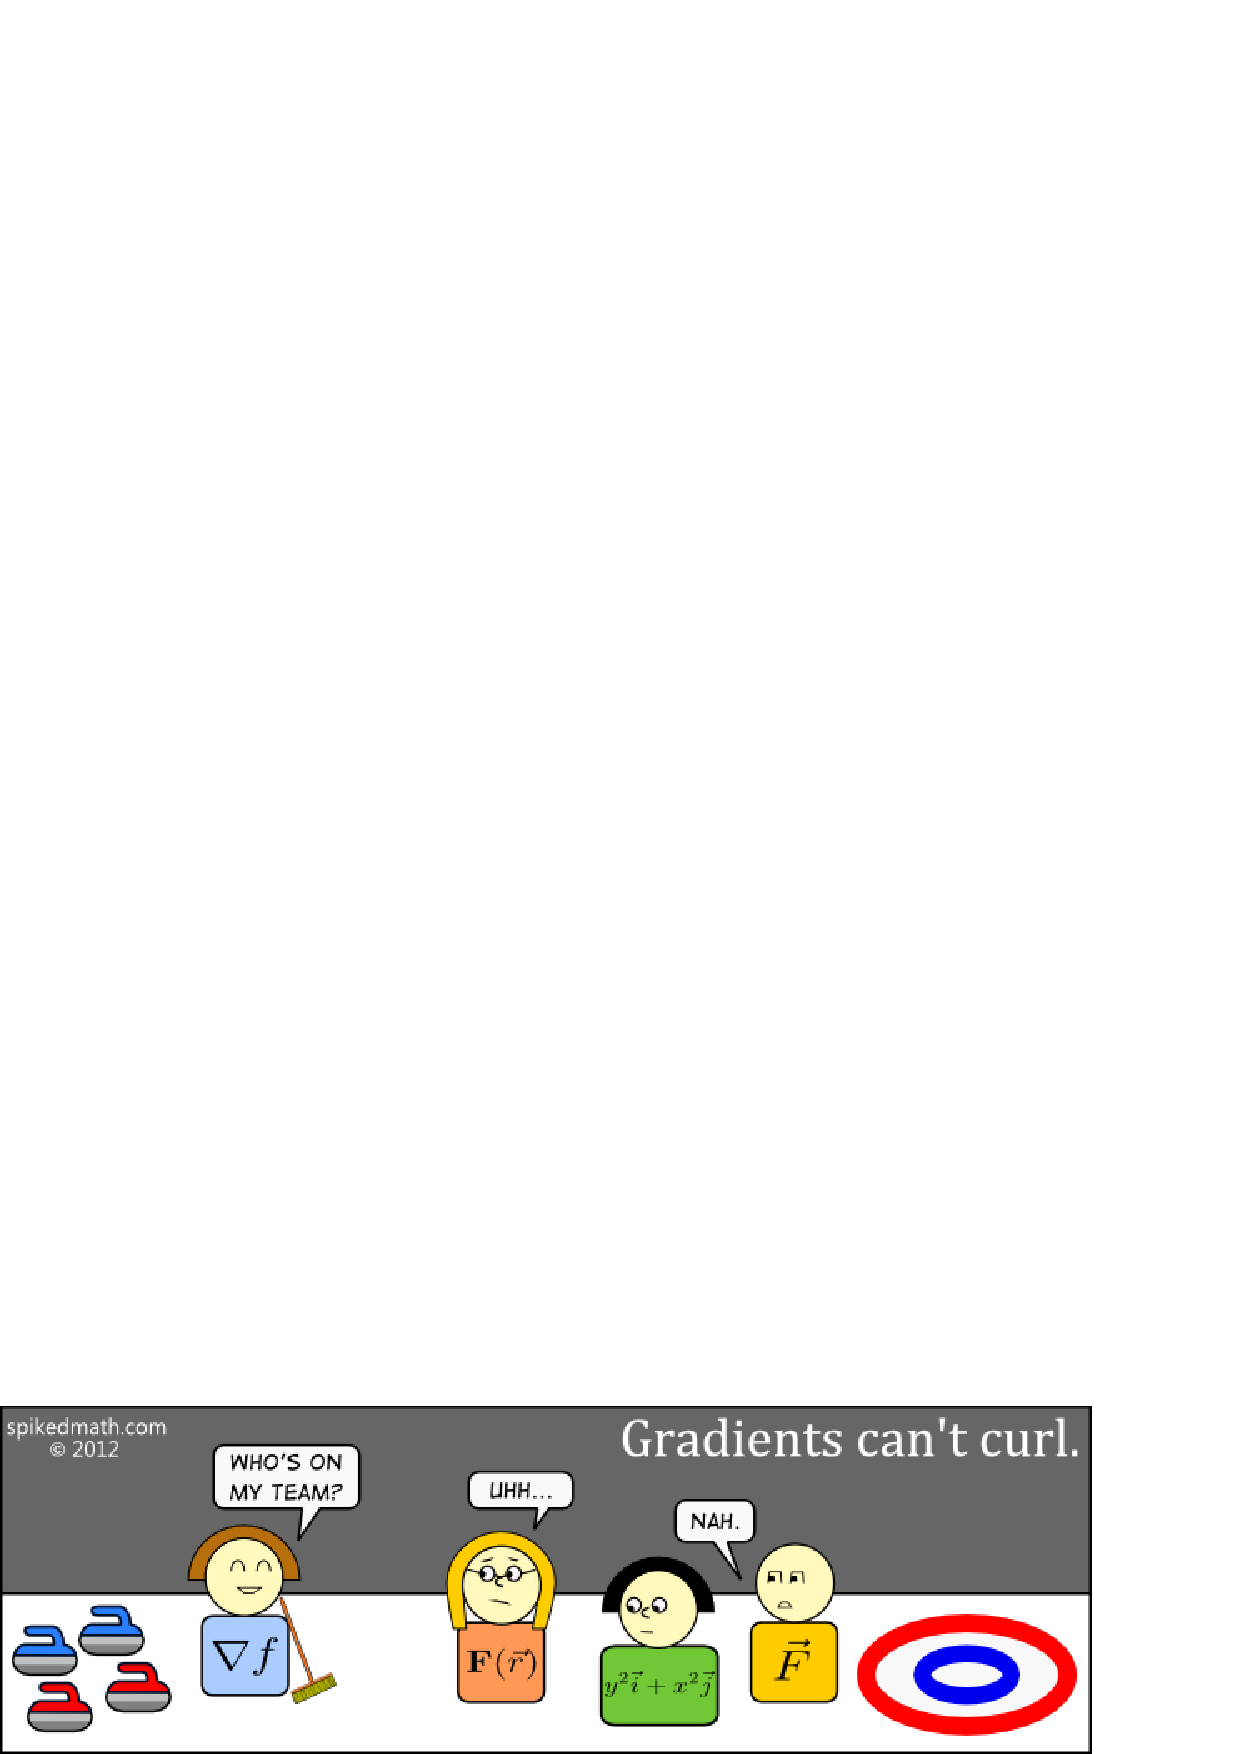
\includegraphics[width=10cm]{pictures_bitmap/501-curling-with-gradients.png}\\
		\url{http://spikedmath.com/501.html}{Spiked math}, \href{http://creativecommons.org/licenses/by-nc-sa/2.5/ca/}{licence Creative Commons by-nc 2.5}.
	\end{center}
}{}

%+++++++++++++++++++++++++++++++++++++++++++++++++++++++++++++++++++++++++++++++++++++++++++++++++++++++++++++++++++++++++++
\section[Interprétation de la divergence]{Interprétation géométrique et physique de la divergence}
%+++++++++++++++++++++++++++++++++++++++++++++++++++++++++++++++++++++++++++++++++++++++++++++++++++++++++++++++++++++++++++

En physique, on dit qu'un champ de vecteurs à divergence nulle est \defe{incompressible}{incompressible!champ de vecteur}. Nous allons essayer de comprendre pourquoi. Lorsqu'un fluide incompressible se déplace, il faut qu'en chaque point il y ait autant de fluide qui rentre que de fluide qui sort. Nous allons voir sur quelques exemples que la divergence d'un champ de vecteurs est le «bilan de masse» d'un fluide qui se déplace selon le champ de vecteurs.

Si en un point la divergence est positive, cela signifie qu'il y a une perte de masse et si la divergence est négative, cela signifie qu'il y a une accumulation de masse.

Prenons par exemple un fluide qui se déplace selon le champ de vitesse montré à figure~\ref{LabelFigBEHTooWsdrys}. % From file BEHTooWsdrys
\newcommand{\CaptionFigBEHTooWsdrys}{Le champ de vecteurs \( F(x,y)=\frac{1}{ x }(1,0)\).}
\input{auto/pictures_tex/Fig_BEHTooWsdrys.pstricks}

Étant donné que la vitesse diminue lorsque \( x\) avance, il y a une accumulation de fluide. Regardez en effet la quantité de fluide qui rentre dans le rectangle par rapport à la quantité de fluide qui en sort. Ce champ de vecteurs a pour équation :
\begin{equation}
	F(x,y)=\frac{1}{ x }\begin{pmatrix}
		1 \\
		0
	\end{pmatrix}=\begin{pmatrix}
		1/x \\
		0
	\end{pmatrix}.
\end{equation}
Sa divergence vaut donc
\begin{equation}
	(\nabla\cdot F)(x,y)=\frac{ \partial F_x }{ \partial x }(x,y)+\underbrace{\frac{ \partial F_y }{ \partial y }(x,y)}_{=0}=-\frac{1}{ x^2 }.
\end{equation}
Cette divergence étant négative, il y a bien accumulation de fluide en tout point, et d'autant plus que \( x\) est petit.

\begin{example}     \label{ExamDivFrot}

	Prenons le champ de vecteurs tournant
	\begin{equation}
		F(x,y)=\frac{1}{ \sqrt{x^2+y^2} }\begin{pmatrix}
			y \\
			-x
		\end{pmatrix}
	\end{equation}
	représenté à la figure~\ref{LabelFigYQVHooYsGLHQ}. Cela est un vecteur qui est constamment perpendiculaire au rayon.


	\newcommand{\CaptionFigYQVHooYsGLHQ}{Le champ de vecteurs \( F(x,y)=(y,-x)\).}
	\input{auto/pictures_tex/Fig_YQVHooYsGLHQ.pstricks}

	Un fluide dont la vitesse serait donné par ce champ de vecteur se contente de tourner. Intuitivement il ne devrait pas y avoir de divergence parce qu'il n'y a aucune accumulation de fluide. En effet,
	\begin{equation}
		\nabla\cdot F(x,y)=\frac{ -2xy }{ (x^2+y^2)^2 }+\frac{ 2xy }{ (x^2+y^2)^2 }=0.
	\end{equation}
\end{example}

\begin{example}
	Prenons le cas du champ de force de gravitation :
	\begin{equation}
		F(x,y,z)=\frac{1}{ (x^2+y^2+z^2)^{3/2} }\begin{pmatrix}
			x \\
			y \\
			z
		\end{pmatrix}.
	\end{equation}
	Nous pouvons rapidement remarquer que \( \nabla\cdot F=0\). Est-ce que cela peut se comprendre sur le dessin de la figure~\ref{LabelFigZGUDooEsqCWQ} ? % From file ZGUDooEsqCWQ
	\newcommand{\CaptionFigZGUDooEsqCWQ}{Le champ de vecteur de la gravité. Nous avons tracé, sur les deux cercles la même densité de vecteurs, c'est-à-dire le même nombre de vecteurs par unité de surface.}
	\input{auto/pictures_tex/Fig_ZGUDooEsqCWQ.pstricks}

	Essayons de voir combien de fluide entre dans la zone bleue et combien en sort. D'abord, il est certain que les vecteurs qui sortent sont plus courts que ceux qui rentrent, ce qui voudrait dire qu'il y a plus de fluide qui rentre. Mais on voit également que le \emph{nombre} de vecteurs qui sortent est plus grand parce que la seconde sphère est plus grande et qu'il y a un vecteur en chaque point de la sphère.

	Intuitivement nous pouvons dire que la quantité qui rentre dans la sphère de rayon \( r_1\) donnée par la taille des vecteurs entrants multiplié par la surface de la sphère, c'est-à-dire
	\begin{equation}        \label{EqQpinormeVecto}
		4\pi r_1^2\| F(x,y,z) \|,
	\end{equation}
	mais \( \| F(x,y,z) \|=\frac{1}{ r_1^2 }\), donc la quantité de fluide entrant est \( 4\pi\). La quantité de fluide sortant sera la même.

	Cela explique deux choses
	\begin{enumerate}
		\item
		      Pourquoi les forces de gravitation et électromagnétiques sont en \( 1/r^2\); c'est parce que nous vivons dans un monde avec trois dimensions d'espace. En étudiant très précisément le champ de gravitation, certains physiciens espèrent trouver des déviations expérimentales par rapport à la règle du \( 1/r^2\); cela \emph{pourrait} être un signe que l'espace contient des dimensions supplémentaires.
		\item
		      Pourquoi il y a un \( 4\pi\) comme coefficient dans beaucoup d'équations en électromagnétisme; en particulier dans certaines anciennes unités de flux.
	\end{enumerate}

\end{example}

\begin{remark}
	Nous allons voir plus loin comment s'assurer que l'équation \eqref{EqQpinormeVecto} représente bien la «quantité de fluide» qui rentre dans la zone délimitée
\end{remark}

%+++++++++++++++++++++++++++++++++++++++++++++++++++++++++++++++++++++++++++++++++++++++++++++++++++++++++++++++++++++++++++
\section{Quelques formules de Leibniz}
%+++++++++++++++++++++++++++++++++++++++++++++++++++++++++++++++++++++++++++++++++++++++++++++++++++++++++++++++++++++++++++

La divergence étant une combinaison de dérivées, il n'est pas tellement étonnant que la divergence de produits donne lieux à des formules en deux termes. Si \( f\) est une fonction et si \( F\) et \( G\) sont des champs de vecteurs, nous avons la proposition suivante.

\begin{proposition}     \label{PROPooDMWEooNaJBCM}
	Si \( F\) et \( G\) sont des champs de vecteurs dont toutes les dérivées partielles existent, alors
	\begin{enumerate}
		\item
		      \( \nabla\cdot(fF)=f\nabla\cdot F+F\cdot\nabla f\)
		\item
		      \( \nabla\cdot(F\times G)=G\cdot\nabla\times F-F\cdot\nabla\times G\)
		\item       \label{ITEMooFDJIooKTnvKj}
		      \( \nabla\times(fF)=f\nabla\times F+\nabla f\times F\).
	\end{enumerate}
\end{proposition}
